\documentclass[a4paper]{article}
\usepackage{cmap}
\usepackage[utf8]{inputenc}
\usepackage[T2A]{fontenc}
\usepackage[english,russian]{babel} 
\usepackage[left=15mm, top=15mm, right=15mm, bottom=42mm, nohead, nofoot]{geometry}
\usepackage{blindtext}  % рыба-текст
\usepackage{graphicx}  % изобржаения
\usepackage{float} % плавающие объекты
\usepackage{wrapfig}  % изобржаения
\usepackage{tikz} % графика
\usepackage{xcolor} % определение цветов
\usepackage{nicefrac} % красивые дроби
\usepackage{cancel} % сокращение
\usepackage{amsmath,amsfonts,amssymb} % математический пакет
\usepackage{hyperref}  % гиперссылки
\usepackage{fancybox,fancyhdr} % хедер и футер
\usepackage{listings} % код
\usepackage{accsupp}
\usepackage{caption}
\captionsetup[figure]{name=Рисунок}
\pagestyle{fancy}
\fancyhf{}
\fancyhead[L]{Лабораторная работа №4}
\fancyhead[R]{\textit{Точностные свойства системы, астатизмы и регуляторы}}
\fancyfoot[C]{\thepage}
\headsep=8mm
\footskip=20mm

\definecolor{urlcolor}{HTML}{3454D1}
\definecolor{linkcolor}{HTML}{3454D1}
\hypersetup{pdfstartview=FitH, linkcolor=linkcolor, urlcolor=urlcolor, colorlinks=true}

\definecolor{strings}{rgb}{0,0.6,0}
\definecolor{comments}{rgb}{0,0.3,0}
\definecolor{numbers}{rgb}{0.5,0.5,0.5}
\definecolor{keywords}{rgb}{0.09,0.61,0.95}
\definecolor{background}{rgb}{0.97,0.97,0.97}
\newcommand{\noncopynumber}[1]{%
    \BeginAccSupp{method=escape,ActualText={}}%
    #1%
    \EndAccSupp{}%
}
\lstdefinestyle{codestyle}{
    backgroundcolor=\color{background},
    commentstyle=\color{comments},
    keywordstyle=\color{keywords},
    stringstyle=\color{strings},
    numberstyle=\tiny\color{numbers}\noncopynumber,
    basicstyle=\ttfamily\footnotesize,
    breakatwhitespace=false,
    breaklines=true,
    captionpos=b,
    inputencoding=utf8,
    keepspaces=true,
    numbers=left,
    numbersep=5pt,
    showspaces=false,
    showstringspaces=false,
    showtabs=false,
    tabsize=2,
    extendedchars=true,
    literate=
    {а}{{\cyra}}1
    {б}{{\cyrb}}1
    {в}{{\cyrv}}1
    {г}{{\cyrg}}1
    {д}{{\cyrd}}1
    {е}{{\cyre}}1
    {ж}{{\cyrzh}}1
    {з}{{\cyrz}}1
    {и}{{\cyri}}1
    {й}{{\cyrishrt}}1
    {к}{{\cyrk}}1
    {л}{{\cyrl}}1
    {м}{{\cyrm}}1
    {н}{{\cyrn}}1
    {о}{{\cyro}}1
    {п}{{\cyrp}}1
    {р}{{\cyrr}}1
    {с}{{\cyrs}}1
    {т}{{\cyrt}}1
    {у}{{\cyru}}1
    {ф}{{\cyrf}}1
    {х}{{\cyrh}}1
    {ц}{{\cyrc}}1
    {ч}{{\cyrch}}1
    {ш}{{\cyrsh}}1
    {щ}{{\cyrshch}}1
    {ъ}{{\cyrhrdsn}}1
    {ы}{{\cyrery}}1
    {ь}{{\cyrsftsn}}1
    {э}{{\cyrerev}}1
    {ю}{{\cyryu}}1
    {я}{{\cyrya}}1
    {А}{{\CYRA}}1
    {Б}{{\CYRB}}1
    {В}{{\CYRV}}1
    {Г}{{\CYRG}}1
    {Д}{{\CYR96}}1
    {Е}{{\CYRE}}1
    {Ж}{{\CYRZH}}1
    {З}{{\CYRZ}}1
    {И}{{\CYRI}}1
    {Й}{{\CYRISHRT}}1
    {К}{{\CYRK}}1
    {Л}{{\CYRL}}1
    {М}{{\CYRM}}1
    {Н}{{\CYRN}}1
    {О}{{\CYRO}}1
    {П}{{\CYRP}}1
    {Р}{{\CYRR}}1
    {С}{{\CYRS}}1
    {Т}{{\CYRT}}1
    {У}{{\CYRU}}1
    {Ф}{{\CYRF}}1
    {Х}{{\CYRH}}1
    {Ц}{{\CYRC}}1
    {Ч}{{\CYRCH}}1
    {Ш}{{\CYRSH}}1
    {Щ}{{\CYRSHCH}}1
    {Ъ}{{\CYRHRDSN}}1
    {Ы}{{\CYRERY}}1
    {Ь}{{\CYRSFTSN}}1
    {Э}{{\CYREREV}}1
    {Ю}{{\CYRYU}}1
    {Я}{{\CYRYA}}1
}

\lstset{style=codestyle}

\addto\captionsrussian{
  \renewcommand{\contentsname}
    {\centering Содержание}
}


\newlength{\tempheight}
\newcommand{\Let}{
\mathbin{\text{\settoheight{\tempheight}{\mathstrut}\raisebox{0.4\pgflinewidth}{
\tikz[baseline=0.5ex,line cap=round,line join=round] \draw (0,0) --++ (0.3em,0) --++ (0,2.3ex) --++ (-0.3em,0);
}}}}
\newcommand*\squared[1]{\tikz[baseline=(char.base)]{
            \node[shape=rectangle,draw,inner sep=4pt] (char) {#1};}}
\newcommand*\msquared[1]{\tikz[baseline=(char.base)]{
            \node[shape=rectangle,draw,inner sep=4pt] (char) {$\displaystyle #1$};}}
\newcommand{\at}{\biggr\rvert}
\newcommand{\shiftright}[3]{\makebox[#2][r]{\makebox[#1][l]{#3}}}
\newcommand{\e}{\;\text{e}}
\let\oldint\int
\def\int{\oldint\limits}
\DeclareRobustCommand{\divby}{%
  \mathrel{\vbox{\baselineskip.65ex\lineskiplimit0pt\hbox{.}\hbox{.}\hbox{.}}}%
}

\newcommand\NB{\textbf{N\kern-0.32em\textcolor{red}{B}}}

\begin{document}

\begin{titlepage}
    \begin{center}
        Федеральное государственное автономное образовательное \\ учреждение высшего образования \\[6pt]
        САНКТ-ПЕТЕРБУРГСКИЙ НАЦИОНАЛЬНЫЙ \\ ИССЛЕДОВАТЕЛЬСКИЙ УНИВЕРСИТЕТ ИТМО \\[16pt]
        Факультет систем управления и робототехники \\[26em]
        Лабораторная работа №4\\[0.5em]
        \textbf{ТОЧНОСТНЫЕ СВОЙСТВА СИСТЕМ, АСТАТИЗМЫ И РЕГУЛЯТОРЫ}
    \end{center}\,\\[10em]
    \begin{flushright}
        Студент: Заводин Е.Ю.\\
        Лин САУ R23 бак 1.1.1 \\[0.5em]
        Преподаватели: Перегудин А.А.\\
        Пашенко А.В.
    \end{flushright}\,\\[6em]
    \begin{center}
        {\small Санкт-Петербург \\ 2025}
    \end{center}
\end{titlepage}
\setcounter{page}{2}
\tableofcontents\newpage

\section{Задача стабилизации с идеальным дифференцирующим звеном}\

В задании рассматривается система 

$$\ddot{y}-\dot{y}+5y=u,$$
корни её характеристического полинома --- $\frac{1\pm\sqrt{19}i}{2}$.\ 

Зададим начальное условие $\dot{y}(0)=5$, промоделируем свободное движение разомкнутой системы ($u=0$):

\begin{figure}[H]
    \centering
    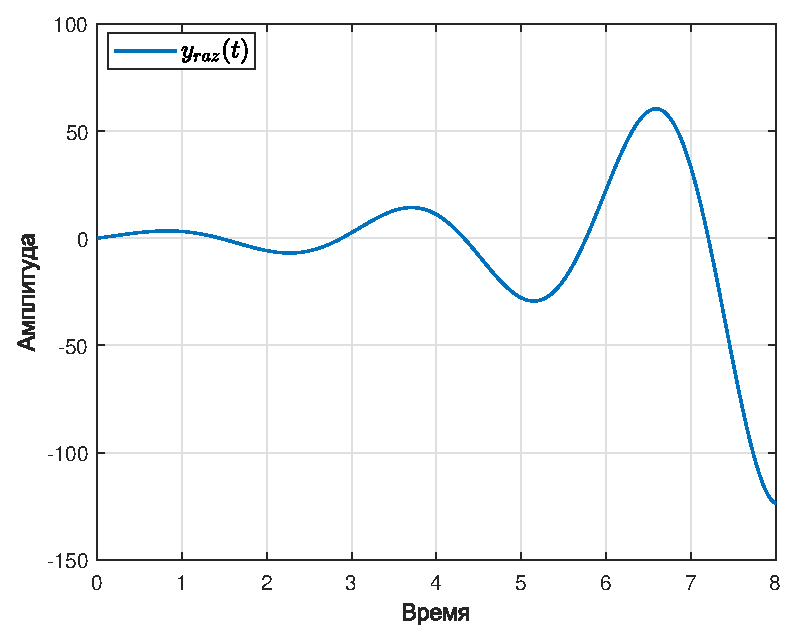
\includegraphics[width=0.6\linewidth]{ex1/razomk_fig.eps}
    \caption{Движение разомкнутой системы}
\end{figure}\

Заметно неустойчивое движение системы. Дабы устранить его, воспользуемся регулятором вида 

$$
u = k_0y + k_1\dot{y}.
$$\

Для моделирования движения системы с воздействием регулятора построим соответствующую структурную схему:

\begin{figure}[H]
    \centering
    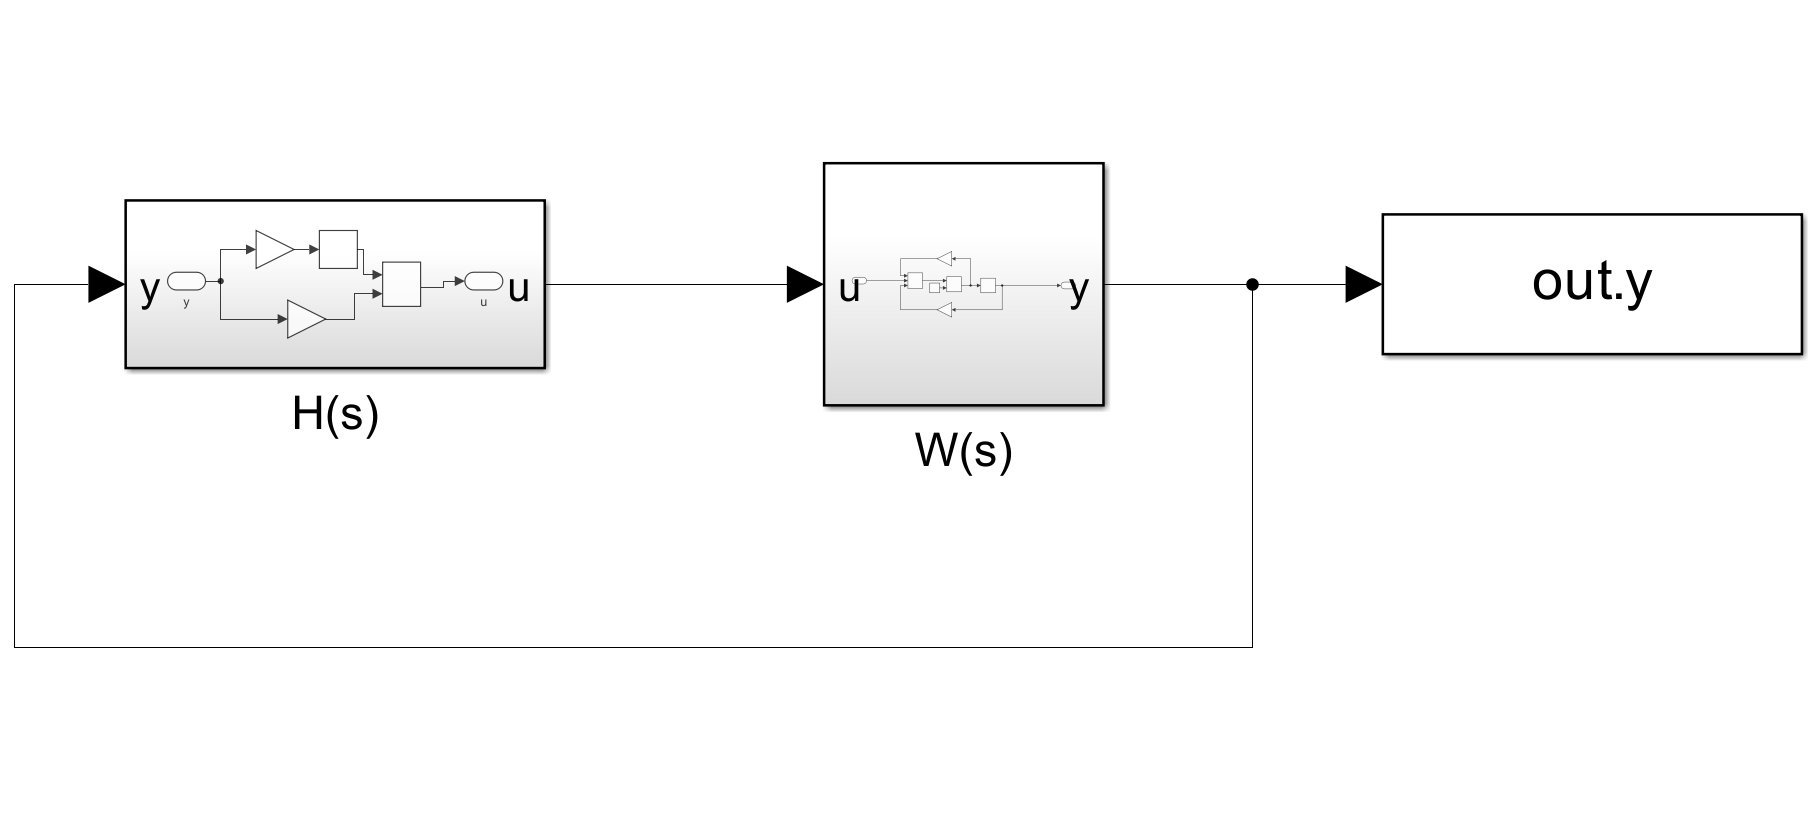
\includegraphics[width=0.65\linewidth]{ex1/scheme_main.png}
    \caption{Структурная схема системы, замкнутой регулятором}
\end{figure}\

\begin{figure}[H]
    \centering
    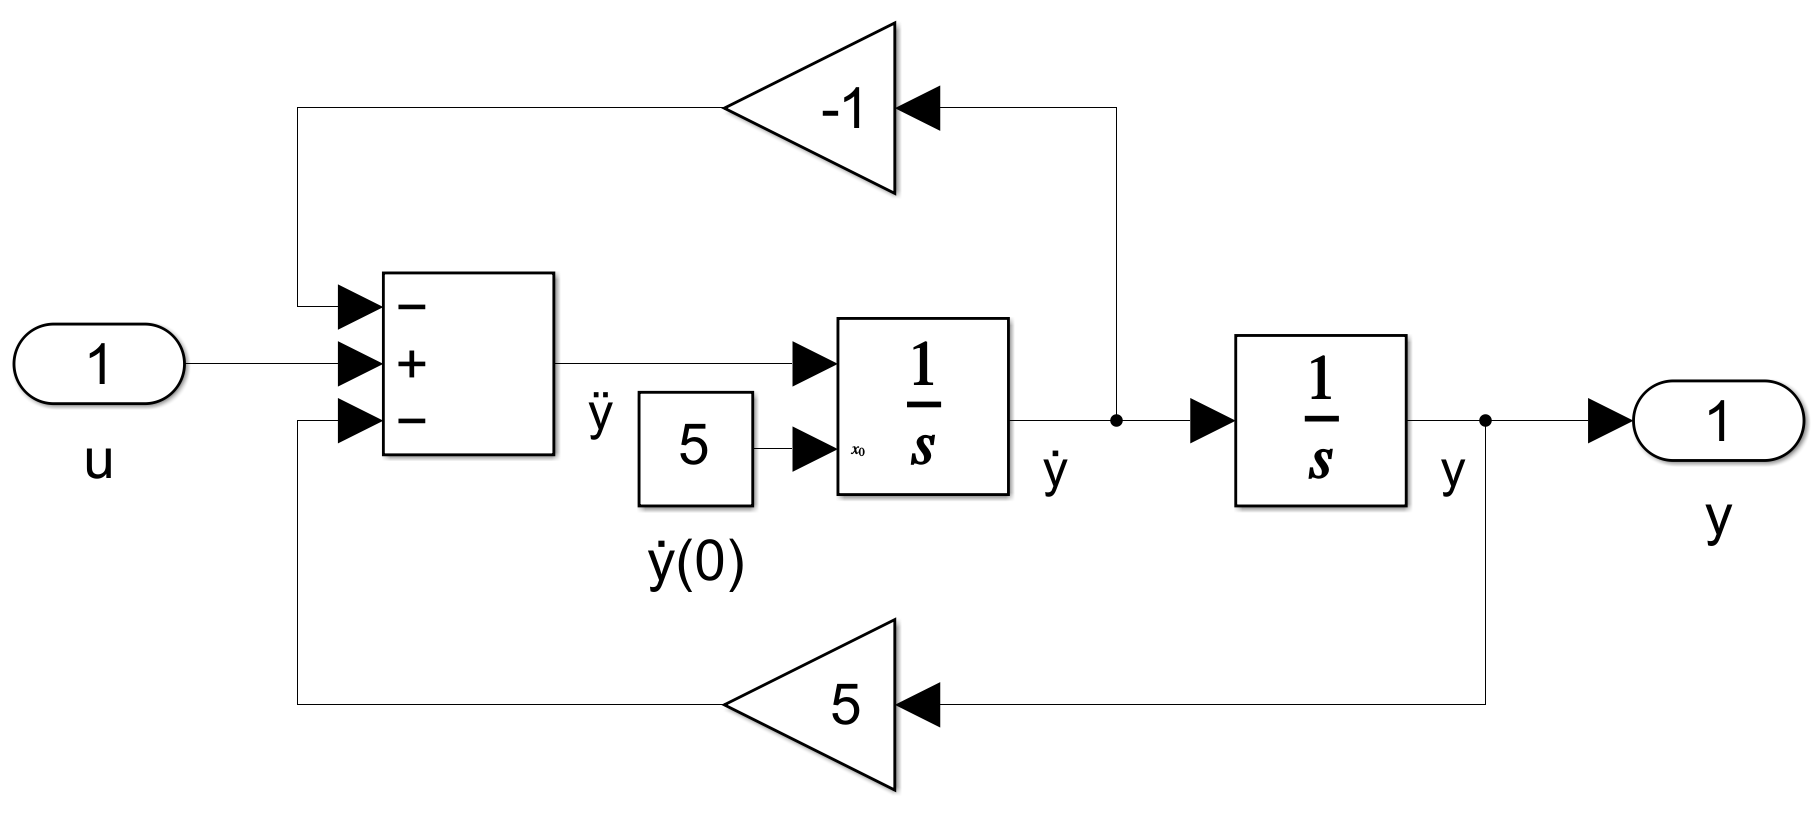
\includegraphics[width=0.65\linewidth]{ex1/scheme_ws.png}
    \caption{Структурная схема объекта управления}
\end{figure}\

\begin{figure}[H]
    \centering
    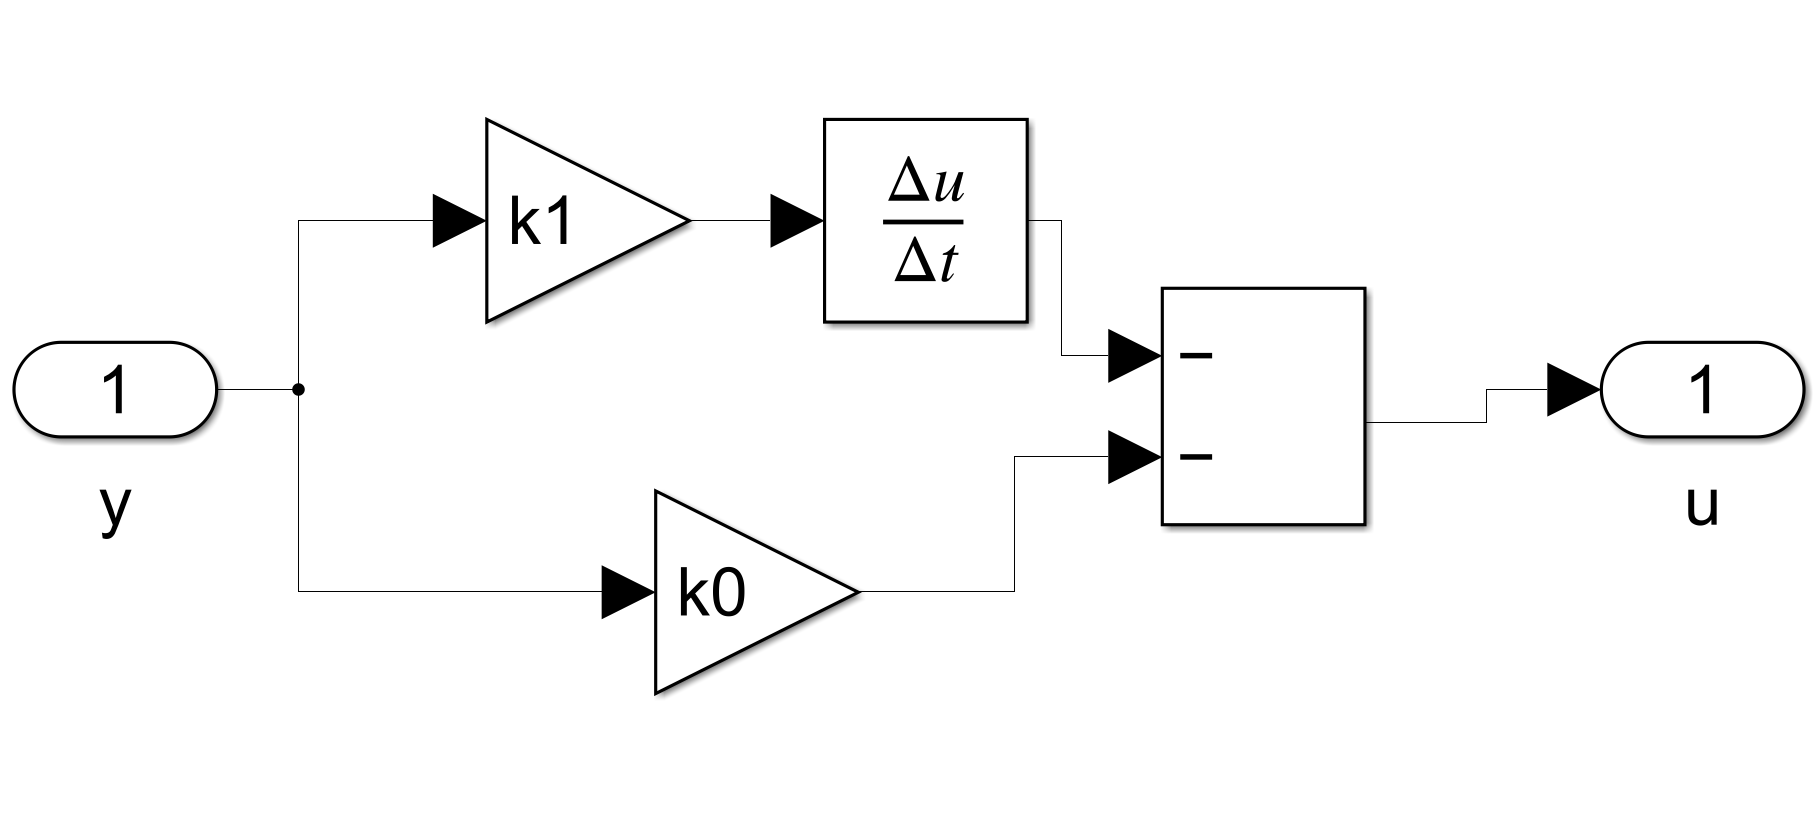
\includegraphics[width=0.65\linewidth]{ex1/scheme_hs.png}
    \caption{Структурная схема регулятора}
\end{figure}\

Чтобы понять, какие значения $k_1, k_0$ выбрать для стабилизации движения системы, проанализируем передаточную функцию, получающуюся после воздействия регулятора.\ 

Передаточную функцию регулятора $W_{\text{рег}}(s)$ в действии на ПФ объекта управления $W_{\text{об}}(s)$ можно рассматривать как отдельную передаточную функцию замкнутой системы:

$$
W(s) = W_{\text{об}}(s)W_{\text{рег}}(s),
$$

$$
Y(s) = \frac{W(s)}{1+W(s)}.
$$\

Устойчивость линейной системы определяется расположением её полюсов: система устойчива, если все полюса лежат в левой полуплоскости комплексной плоскости. Полюса замкнутой системы --- корни знаменателя этой дроби, то есть решения уравнения

$$
1 + W(s) = 0 \Leftrightarrow 1 + W_{\text{об}}(s)W_{\text{рег}}(s) = 0.
$$

$$
\ddot{y} - \dot{y} + 5y = u \Leftrightarrow s^2y-sy+5y = u \Leftrightarrow y = \left(\frac{1}{s^2-s+5}\right)u \Rightarrow W_{\text{об}}(s) = \frac{1}{s^2-s+5}
$$

$$
u = k_0 y+k_1\dot{y} \Leftrightarrow u = k_0y + k_1sy \Leftrightarrow u = y(k_0 + k_1s) \Rightarrow W_{\text{рег}}(s) = k_0 + k_1s
$$

$$
1 + W_{\text{об}}(s)W_{\text{рег}}(s) = 1 + \frac{k_0 + k_1s}{s^2-s+5} = 1(s^2-s+5) + k_0+k_1s = s^2 + (k_1-1)s+(k_0+5)=0
$$\ 

Система будет асимптотически устойчива, если $k_0+5 > 0 \Leftrightarrow k_0 > -5$ и $k_1-1 > 0 \Leftrightarrow k_1 > 1$. При $k_0 = -5, k_1 = 1$ система устойчива по Ляпунову.\ 

Примем $k_0 = 1, k_1 = 3$, промоделируем систему при таких значениях параметров:

\begin{figure}[H]
    \centering
    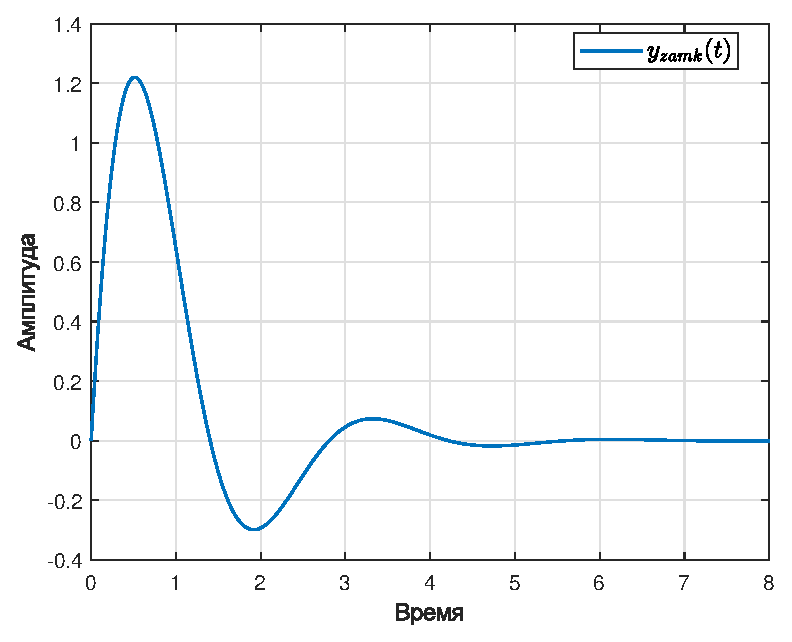
\includegraphics[width=0.65\linewidth]{ex1/zamk_fig.eps}
    \caption{Движение системы, замкнутой регулятором}
\end{figure}\

Видим, что теперь система асимптотически устойчива с установившимся значением $y_{\text{уст}} = 0$, таким образом получилось стабилизировать неустойчивую разомкнутую систему действием на неё регулятора.

\section{Задача стабилизации с реальным дифференцирующим звеном}\

В задании аппроксимация производной при помощи блока $\text{Derivative}$ заменяется передаточной функцией

$$
W_{\text{р.дифф.}}(p) = \frac{p}{Tp+1}.
$$\

Это значит, что меняется и передаточная функция $W_{\text{рег}}(s)$, с учётом введения в него новой передаточной функции он начинает выглядеть следующим образом:

$$
W_{\text{рег}} = k_0+k_1\frac{s}{Ts+1}.
$$\ 

Проанализируем, при каких $T$ система будет неустойчива, по аналогии с предыдущим заданием воспользовавшись анализом корней знаменателя передаточной функции замкнутой системы:

$$
W(s) = \left(k_0 + k_1 \frac{s}{T s + 1}\right) \cdot \frac{1}{s^2 - s + 5} = \frac{(k_0 T + k_1)s + k_0}{T s + 1}\cdot \frac{1}{s^2 - s + 5} = \frac{(k_0 T + k_1)s + k_0}{(T s + 1)(s^2 - s + 5)}.
$$\

Тогда
$$
1 + W(s) = 0 \quad \Rightarrow \quad (T s + 1)(s^2 - s + 5) + (k_0 T + k_1)s + k_0 = 0.
$$\ 

Раскроем скобки:  
$$
(T s + 1)(s^2 - s + 5) = T s(s^2 - s + 5) + 1\cdot(s^2 - s + 5)=
$$
$$
= T s^3 - T s^2 + 5T s + s^2 - s + 5=
$$
$$
= T s^3 + (1 - T)s^2 + (5T - 1)s + 5.
$$\

$$
T s^3 + (1-T)s^2 + (5T - 1 + k_0 T + k_1)s + (5 + k_0) = 0.
$$\ 

Подставим выбранные $k_0 = 1, k_1 = 3$:

$$
T s^3 + (1-T)s^2 + (5T + T + 2)s + 6 = 0 \Leftrightarrow s^3 + \frac{1-T}{T}s^2 + \left(\frac{2}{T} + 6\right)s + \frac{6}{T} = 0
$$\

По критерию Гурвица кубический полином устойчив, если $a_2, a_1, a_0 > 0$ и $a_2 a_1 > a_0$. В нашем случае система асимптотически устойчива, если выполнены следующие условия:

$$
a_0 = \frac{6}{T} > 0 \Leftrightarrow T > 0
$$
$$
a_1 = \frac{2}{T} + 6 > 0 \Leftrightarrow T > -\frac{2}{6}, T\neq0
$$
$$
a_2 = \frac{1 - T}{T} > 0 \Leftrightarrow 1 - T > 0, \Leftrightarrow T < 1
$$\ 

$$a_2 a_1 > a_0 \Leftrightarrow
\left(\frac{1 - T}{T}\right) \left(\frac{2}{T} + 6\right) > \frac{6}{T}.
$$\ 

Из условий выше знаем, что $T > 0$, значит, можем домножить на $T$:

\[
(1 - T)\left(\frac{2}{T} + 6\right) > 6.
\]

Раскрывая скобки, получим:

\[
(1 - T)\cdot\frac{2}{T} + (1 - T)\cdot6 > 6\Leftrightarrow
\frac{2(1 - T)}{T} + 6(1 - T) > 6\Leftrightarrow
\]

\[
\frac{2(1 - T)}{T} + 6(1 - T) - 6 > 0\Leftrightarrow
\frac{2(1 - T)}{T} + 6(1 - T - 1) > 0\Leftrightarrow
\frac{2(1 - T)}{T} - 6T > 0.
\]

Приведём к общему знаменателю \(T > 0\):

\[
\frac{2(1 - T) - 6T^2}{T} > 0\Leftrightarrow
\frac{-6T^2 - 2T + 2}{T} > 0.
\]\

Корни числителя:

\[
T_{1, 2} = \frac{-1 \pm \sqrt{13}}{6}.
\]\ 

Ветви соответствующей уравнению параболы направлены вверх, а значит, система неустойчива при $T \ge \frac{-1 + \sqrt{13}}{6}$ и при $T\le \frac{-1 - \sqrt{13}}{6}$.\ Итого, сопоставляя полученные ограничения на $T$, получаем отрезок, в котором система асимптотически устойчива: $T \in \left(0, \frac{-1 + \sqrt{13}}{6}\right)$

Система была промоделирована для нескольких различных значений параметра $T$, соответствующих устойчивой системе:

\begin{figure}[H]
    \centering
    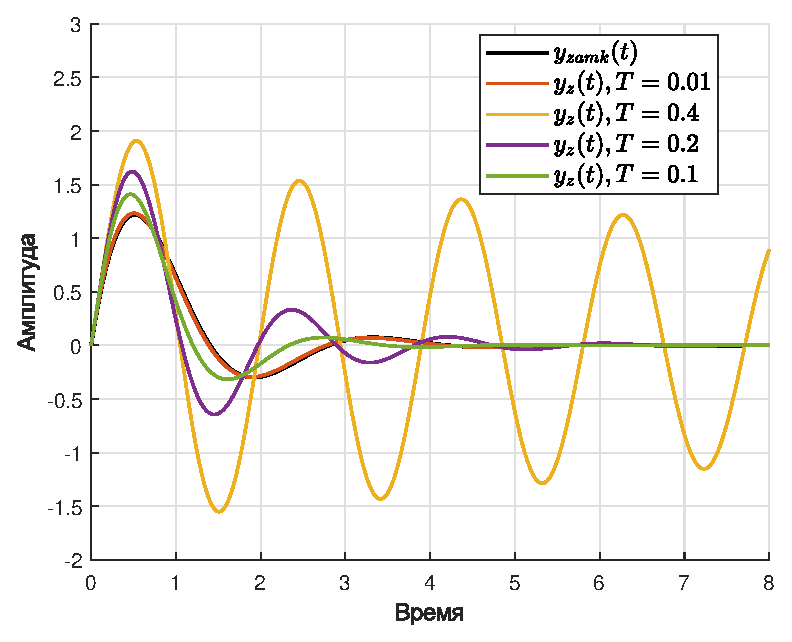
\includegraphics[width=0.65\linewidth]{ex2/all.eps}
    \caption{Движение системы при разных $T$, в сравнении с результатом моделирования из задания 1}
\end{figure}\

Заметно, что чем ближе $T$ к 0, тем ближе соответствующая траектория к траектории $y_{zamk}(t)$, полученной в первом задании. Также чем ближе $T$ к своей верхней границе, тем сильнее расходится траектория движения системы. Отдельно промоделирую систему на верхней границе, $T = \frac{-1 + \sqrt{13}}{6}\approx 0.434$:

\begin{figure}[H]
    \centering
    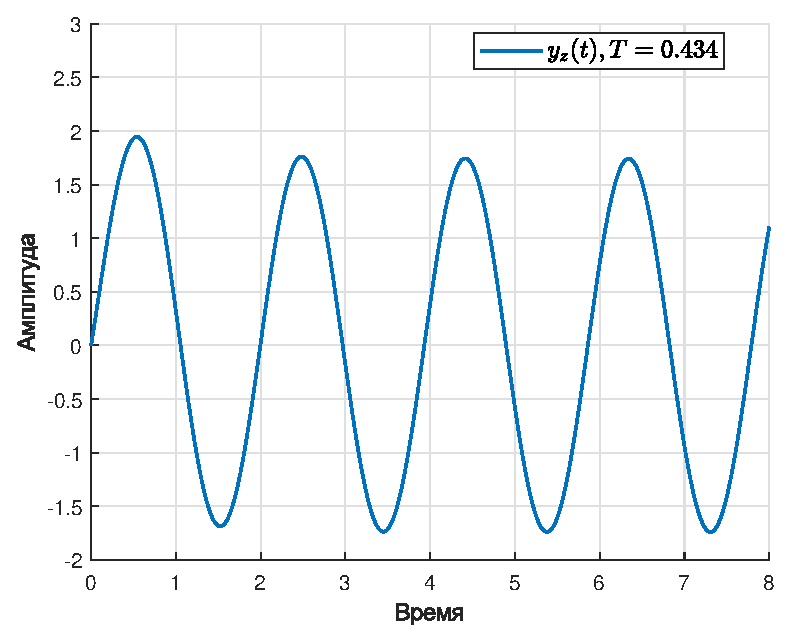
\includegraphics[width=0.65\linewidth]{ex2/0.434.eps}
    \caption{Движение системы при граничном значении $T$}
\end{figure}\

Видно, что траектория движения системы больше походит на устойчивую по Ляпунову, чем на асимптотическую.

\subsection{Вывод}\

Я понял, что добавление в регулятор дифференцирующего звена меняет его передаточную функцию, и понял, как определить устойчивость системы исходя из параметра добавленного звена. 

\section{Задача слежения для системы с астатизмом нулевого порядка (П-регулятор)}\

Рассмотрим замкнутую систему, заданную структурной схемой, отображённой на рисунке:

\begin{figure}[H]
    \centering
    
\includegraphics[width=0.65\linewidth]{ex3/image.png}
    \caption{Структурная схема с П-регулятором}
\end{figure}\

Передаточная функция системы --- $W_s(s) = \frac{5}{s^2+5s+6}$, регулятором выступает $H(s) = k$. Для значения параметра регулятора был выбран набор значений $[1, 3, 7]$.\ 

\subsection{Стационарная желаемая функция}\

Исследование стационарного режима работы проводится с задающим воздействием $g(t) = 1$. Для этого режима при выбранной передаточной функции объекта управления и регулятора можно будет найти установившееся значение ошибки (система обладает нулевым порядком астатизма, а значит, при $t \to \infty$ между траекторией движения системы и задающим воздействием будет фиксированная величина $e_\text{уст}$).\ 

Для расчёта установившейся ошибки понадобится вычислить передаточную функцию разомкнутой системы:

$$
W(s) = W_s(s) H(s) = \frac{5k}{s^2+5s+6}
$$\ 

Зная передаточную функцию разомкнутой системы, можем построить передаточную функцию по ошибке слежения:

$$
\underset{g\to e}{W}(s) = \frac{1}{1+W(s)} = \frac{1}{1+\frac{5k}{s^2+5s+6}}=\frac{s^2+5s+6}{s^2+5s+6+5k}
$$\ 

Тогда образ Лапласа ошибки слежения будет определяться как 

$$
E(s) = \underset{g\to e}{W}(s) \cdot G(s),
$$
где $G(s) = \frac{1}{s}$ -- образ Лапласа от задающего воздействия $g(t) = 1$.

$$
E(s) = \frac{s^2+5s+6}{s(s^2+5s+6+5k)}.
$$\ 

Пользуясь теоремой о конечном значении, можем вычислить непосредственно установившуюся ошибку:

$$
e_{\text{уст}} = \lim_{t\to +\infty} e(t) = \lim_{s\to 0} sE(s) = \lim_{s\to 0}\frac{\cancel{s}\left(s^2+5s+6\right)}{\cancel{s}\left(s^2+5s+6+5k\right)} = \frac{\cancelto{0}{s^2}+5\cancelto{0}{s}+6}{\cancelto{0}{s^2}+5\cancelto{0}{s}+6+5k} =\frac{6}{6+5k}
$$\ 

Тогда для $k = 1$ $e_{\text{уст}} = \frac{6}{11}$, для $k = 3$: $e_{\text{уст}} = \frac{6}{21}$, для $k = 7$: $e_{\text{уст}} = \frac{6}{41}$.\ 

То есть чем больше $k$, тем ближе он к 0.\ 

Проверим теорию на ``практике'':

\begin{figure}[H]
    \begin{minipage}{0.5\textwidth}
        \centering 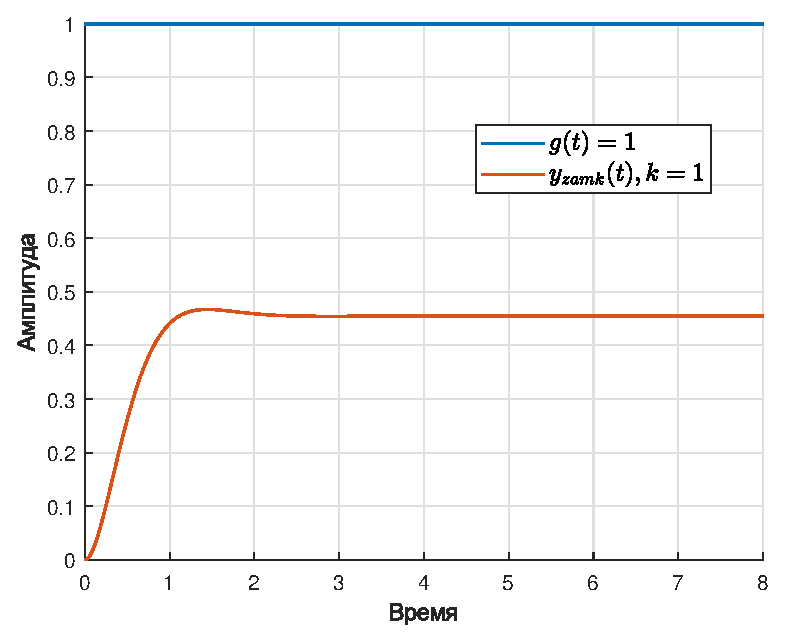
\includegraphics[width=\textwidth]{ex3/k1_g_a.eps}
        \caption{Графики входа и выхода при $k=1$, $g=1$}
    \end{minipage}\hfill
    \begin{minipage}{0.5\textwidth}
        \centering 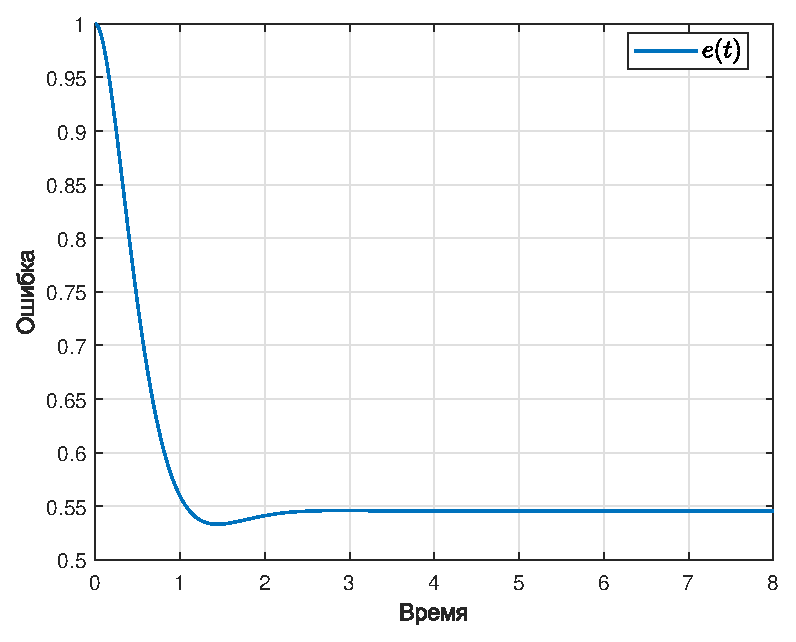
\includegraphics[width=\textwidth]{ex3/k1_g_a_error.eps}
        \caption{График ошибки при $k=1$, $g=1$}
        % \centerline{лягушки}
    \end{minipage}\\[1em]
\end{figure}\noindent\

В этом случае установившаяся ошибка совпадает с предсказанной $e_{\text{уст}} =\frac{6}{11} \approx 0.55$.

\begin{figure}[H]
    \begin{minipage}{0.5\textwidth}
        \centering 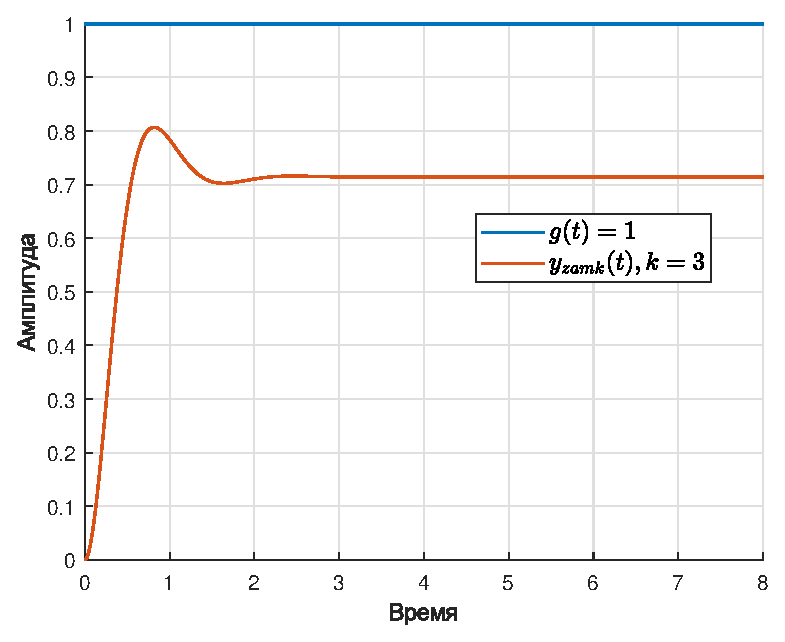
\includegraphics[width=\textwidth]{ex3/k3_g_a.eps}
        \caption{Графики входа и выхода при $k=3$, $g=1$}
    \end{minipage}\hfill
    \begin{minipage}{0.5\textwidth}
        \centering 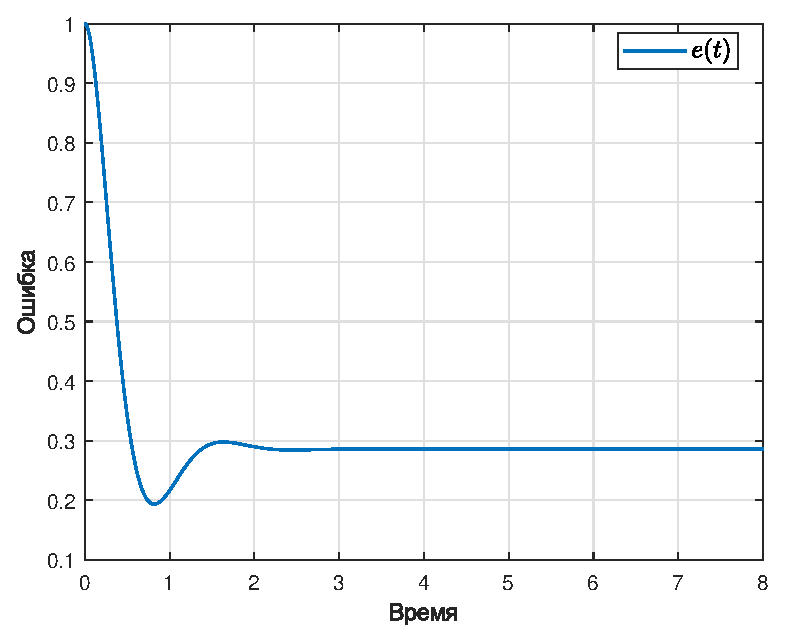
\includegraphics[width=\textwidth]{ex3/k3_g_a_error.eps}
        \caption{График ошибки при $k=3$, $g=1$}
        % \centerline{лягушки}
    \end{minipage}\\[1em]
\end{figure}\noindent\

В этом случае установившаяся ошибка также совпадает с предсказанной $e_{\text{уст}} =\frac{6}{21} \approx 0.29$.

\begin{figure}[H]
    \begin{minipage}{0.5\textwidth}
        \centering 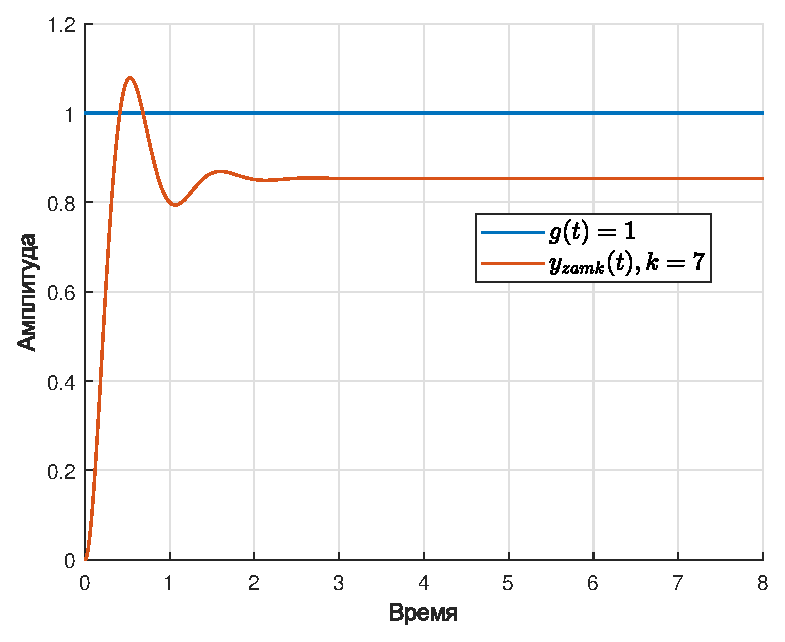
\includegraphics[width=\textwidth]{ex3/k7_g_a.eps}
        \caption{Графики входа и выхода при $k=7$, $g=1$}
    \end{minipage}\hfill
    \begin{minipage}{0.5\textwidth}
        \centering 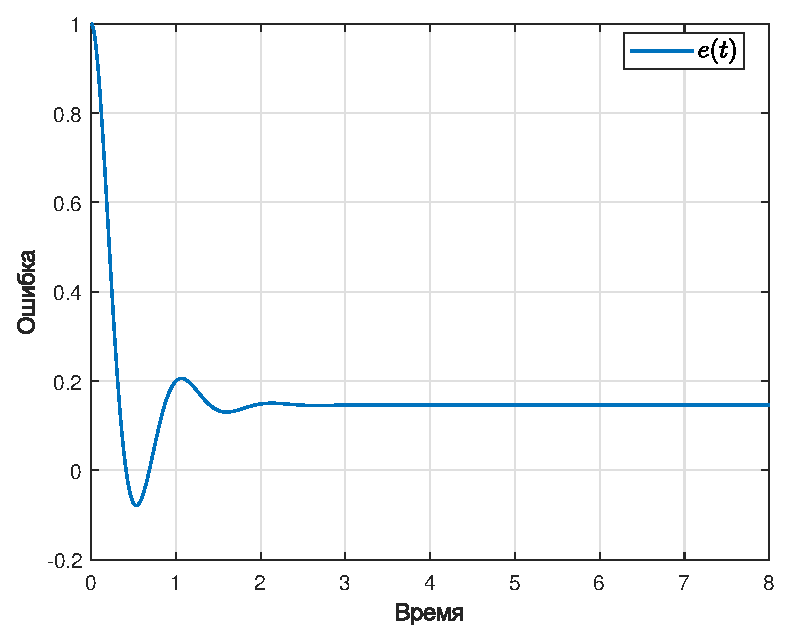
\includegraphics[width=\textwidth]{ex3/k7_g_a_error.eps}
        \caption{График ошибки при $k=7$, $g=1$}
        % \centerline{лягушки}
    \end{minipage}\\[1em]
\end{figure}\noindent\

В этом случае установившаяся ошибка снова совпадала с предсказанной $e_{\text{уст}} =\frac{6}{41} \approx 0.16$.

Во всех трёх случаях ошибка сошлась к константе, как и ожидалось. Заметно, что чем больше $k$, тем меньше установившаяся ошибка, но в то же время и больше перерегулирование, и тем больше колебательности появляется у конечного сигнала.

\subsection{Функция с постоянной скоростью}\

В этой части задания на вход подаётся линейно растущее воздействие -- $g(t) = t$. Из-за низкого порядка астатизма система не сможет ни свести ошибку слежения к 0, ни прийти к установившемуся значению этой ошибки: 

\begin{figure}[H]
    \begin{minipage}{0.5\textwidth}
        \centering 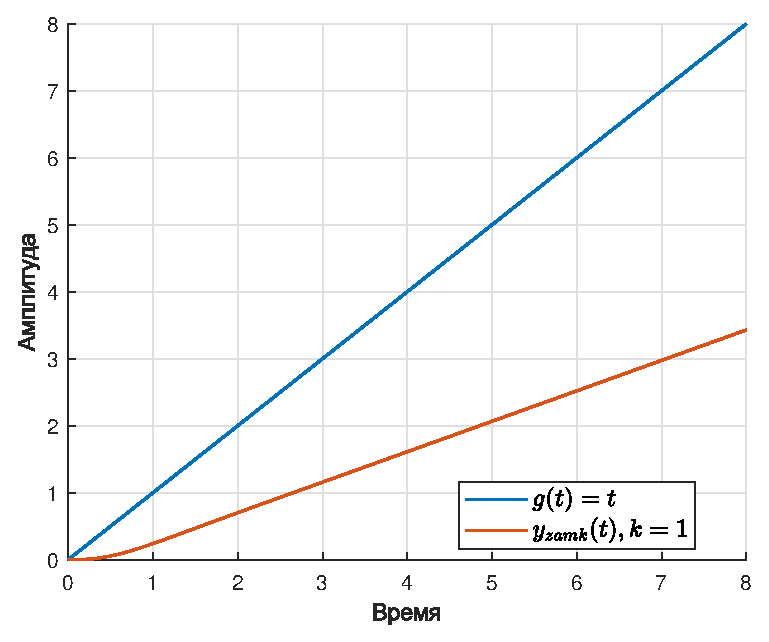
\includegraphics[width=\textwidth]{ex3/k1_g_vt.eps}
        \caption{Графики входа и выхода при $k=1$, $g(t)=1$}
    \end{minipage}\hfill
    \begin{minipage}{0.5\textwidth}
        \centering 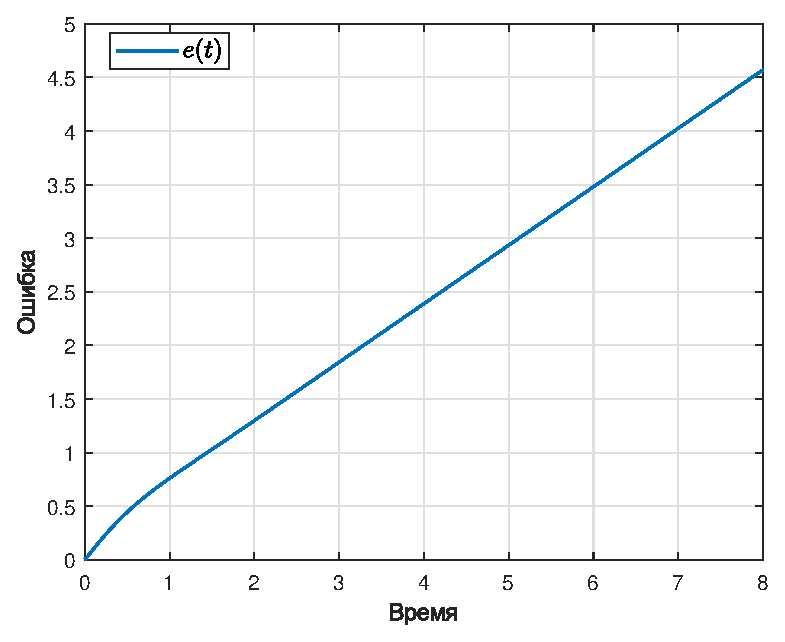
\includegraphics[width=\textwidth]{ex3/k1_g_vt_error.eps}
        \caption{График ошибки при $k=1$, $g(t)=t$}
        % \centerline{лягушки}
    \end{minipage}\\[1em]
\end{figure}\noindent\

\begin{figure}[H]
    \begin{minipage}{0.5\textwidth}
        \centering 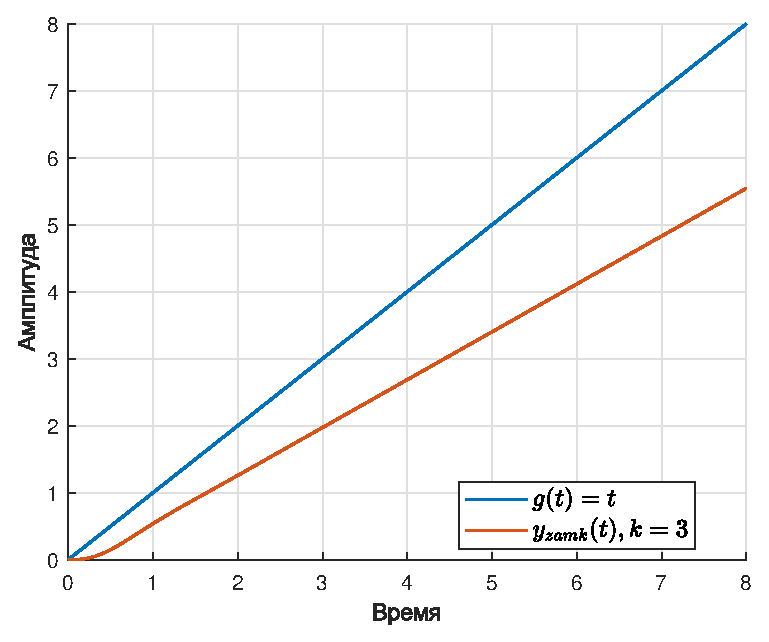
\includegraphics[width=\textwidth]{ex3/k3_g_vt.eps}
        \caption{Графики входа и выхода при $k=3$, $g(t)=t$}
    \end{minipage}\hfill
    \begin{minipage}{0.5\textwidth}
        \centering 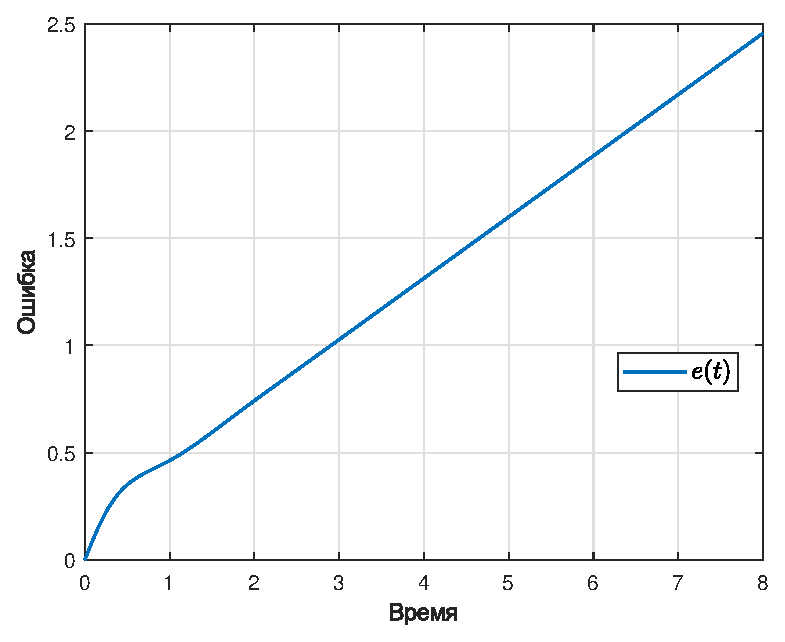
\includegraphics[width=\textwidth]{ex3/k3_g_vt_error.eps}
        \caption{График ошибки при $k=3$, $g(t)=t$}
        % \centerline{лягушки}
    \end{minipage}\\[1em]
\end{figure}\noindent\

\begin{figure}[H]
    \begin{minipage}{0.5\textwidth}
        \centering 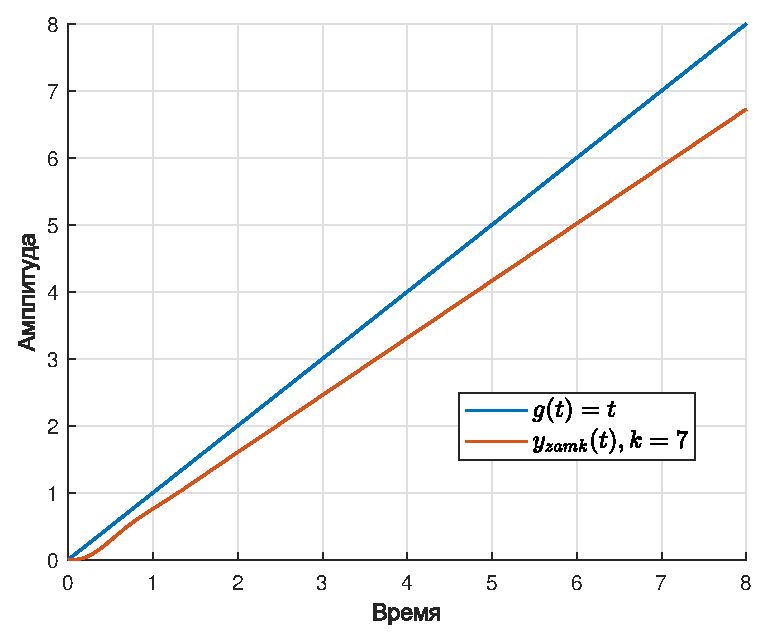
\includegraphics[width=\textwidth]{ex3/k7_g_vt.eps}
        \caption{Графики входа и выхода при $k=7$, $g(t)=t$}
    \end{minipage}\hfill
    \begin{minipage}{0.5\textwidth}
        \centering 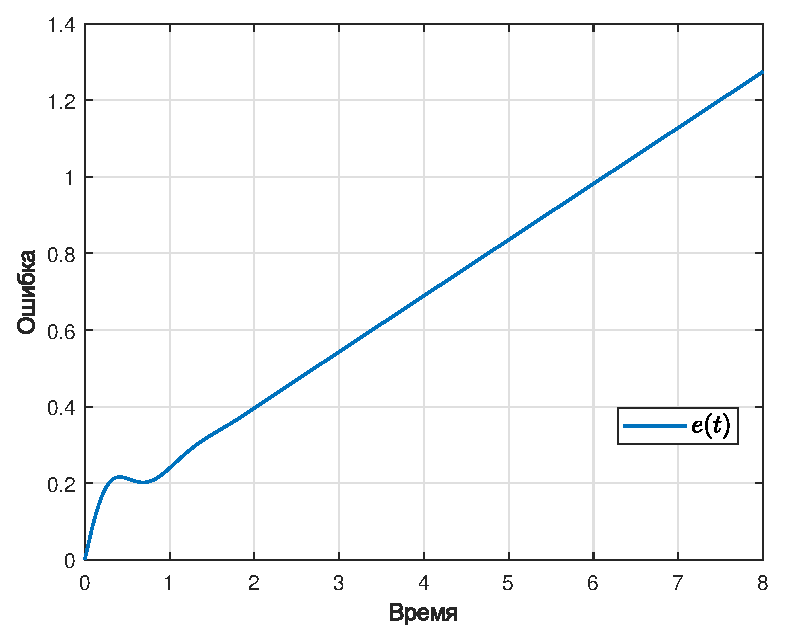
\includegraphics[width=\textwidth]{ex3/k7_g_vt_error.eps}
        \caption{График ошибки при $k=7$, $g(t)=t$}
        % \centerline{лягушки}
    \end{minipage}\\[1em]
\end{figure}\noindent\

Из полученных графиков можно заключить, что чем выше $k$, тем медленнее будет расти ошибка, при $k \to \infty$ ошибка будет стремиться к линейно растущему задающему воздействию. Однако расти будут и колебания, появляющиеся на рисунке для случая $k = 7$.

\subsection{Выводы}\ 

Система, рассмотренная с пропорциональным регулятором, не может полностью ``уследить'' даже за линейным входом, выход отстаёт от входа. Дело в нулевом порядке астатизма - если его увеличить на хотя бы до первого, можно будет добиться постоянного значения установившейся ошибки для случая с линейно растущим входом.

\section{Задача слежения для системы с астатизмом первого порядка (И-регулятор)}\

В задании рассматривается система, заданная структурной схемой, представленной на рисунке:

\begin{figure}[H]
    \centering
    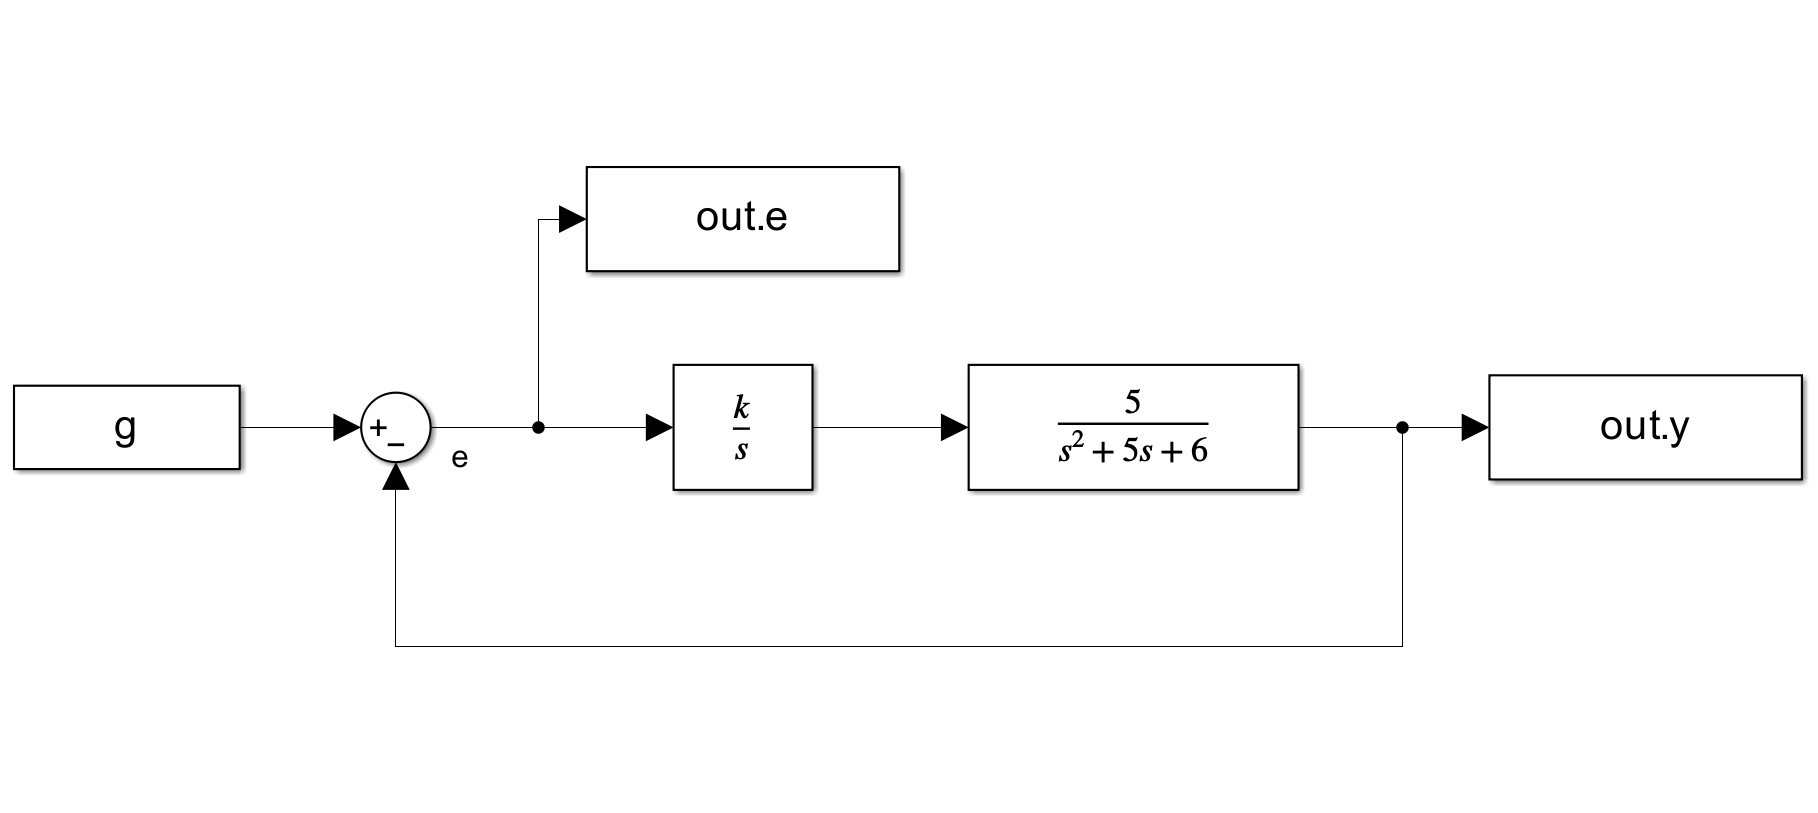
\includegraphics[width=0.65\linewidth]{ex4/scheme.png}
    \caption{Структурная схема с И-регулятором}
\end{figure}\

Это всё та же система, но с интегральным регулятором $(H(s) = \frac{k}{s})$ вместо пропорционального. У регулятора есть параметр $k$, я буду варьировать значения этого параметра из набора $[0.5, 1, 3]$.\ 

Система обладает первым порядком астатизма, а значит, установившаяся ошибка должна свестись к $0$ при $t \to \infty$ в случае константного входа и к константе в случае линейно растущего входа. 

\subsection{Стационарный режим работы, $g(t) = 1$}\

В стационарном режиме ошибка должна прийти к 0 из-за того, что система обладает первым порядком астатизма, это известно из лекции. Однако покажу это явно:\

$$
W(s) = W_{\text{s}}(s) H(s) = \frac{5k}{s(s^2+5s+6)}
$$\

$$
\underset{g\to e}{W}(s) = \frac{1}{1+W(s)} = \frac{1}{1+\frac{5k}{s(s^2+5s+6)}} = \frac{s(s^2+5s+6)}{s(s^2+5s+6) + 5k}
$$

$$
E(s) = \underset{g\to e}{W}(s) \cdot G(s) = \frac{s(s^2+5s+6)}{s(s^2+5s+6) + 5k} \cdot \frac{1}{s} = \frac{s(s^2+5s+6)}{s^2(s^2+5s+6) + 5ks}
$$

$$
e_{\text{уст}} = \lim_{t\to +\infty} e(t) = \lim_{s\to 0} sE(s) = \lim_{s\to 0} \frac{s^2(s^2+5s+6)}{s^2(s^2+5s+6) + 5ks} = \lim_{s\to 0} \frac{\cancelto{0}{s}(\cancelto{0}{s^2}+5\cancelto{0}{s}+6)}{\cancelto{0}{s}(\cancelto{0}{s^2}+5\cancelto{0}{s}+6) + 5k} = \frac{0}{5k} = 0.
$$\

Проведем эксперименты, сравним теорию с симулированной реальностью:

\begin{figure}[H]
    \begin{minipage}{0.5\textwidth}
        \centering 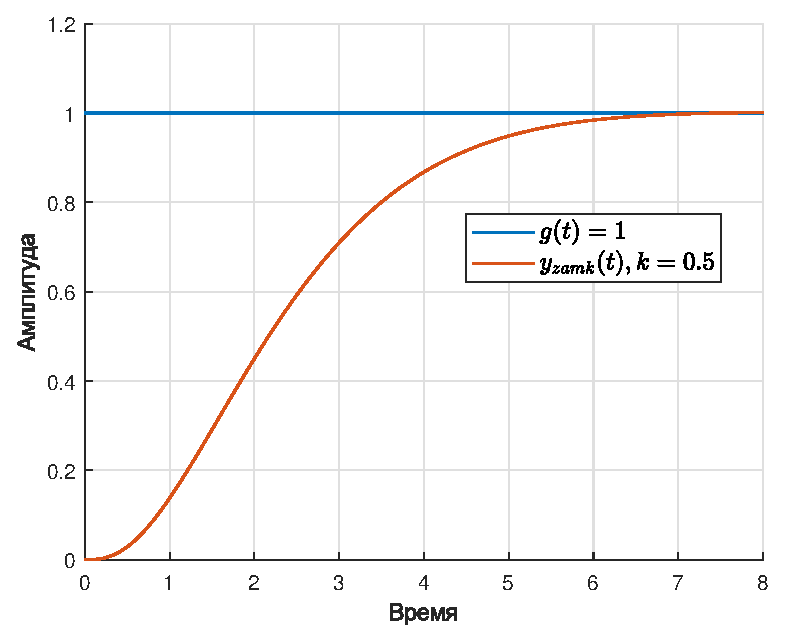
\includegraphics[width=\textwidth]{ex4/k0.5_g_a.eps}
        \caption{Графики входа и выхода при $k=0.5$, $g(t)=1$}
    \end{minipage}\hfill
    \begin{minipage}{0.5\textwidth}
        \centering 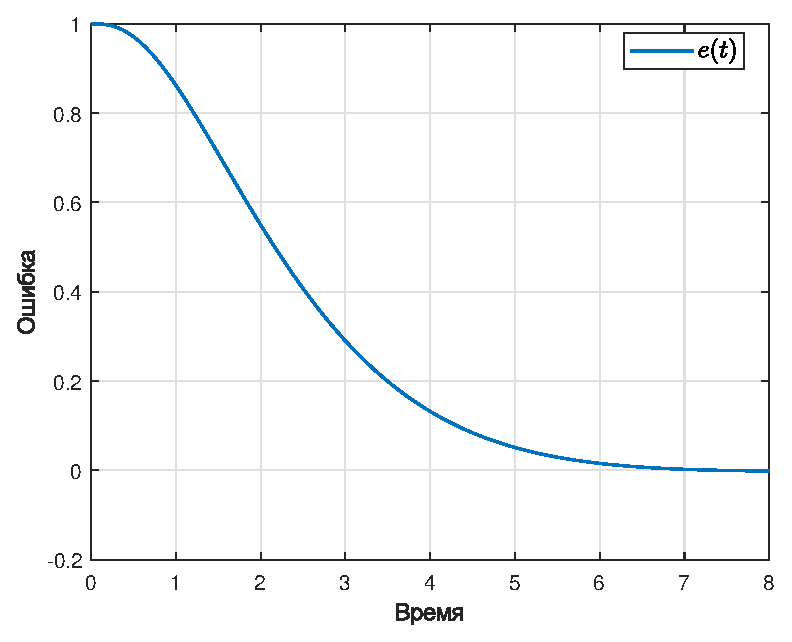
\includegraphics[width=\textwidth]{ex4/k0.5_g_a_error.eps}
        \caption{График ошибки при $k=0.5$, $g(t)=1$}
        % \centerline{лягушки}
    \end{minipage}\\[1em]
\end{figure}\noindent\

\begin{figure}[H]
    \begin{minipage}{0.5\textwidth}
        \centering 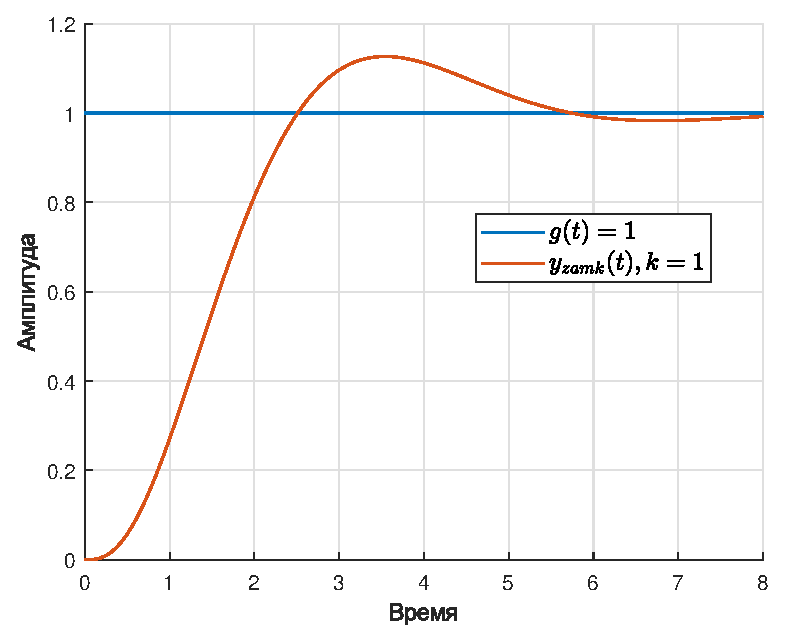
\includegraphics[width=\textwidth]{ex4/k1_g_a.eps}
        \caption{Графики входа и выхода при $k=1$, $g(t)=1$}
    \end{minipage}\hfill
    \begin{minipage}{0.5\textwidth}
        \centering 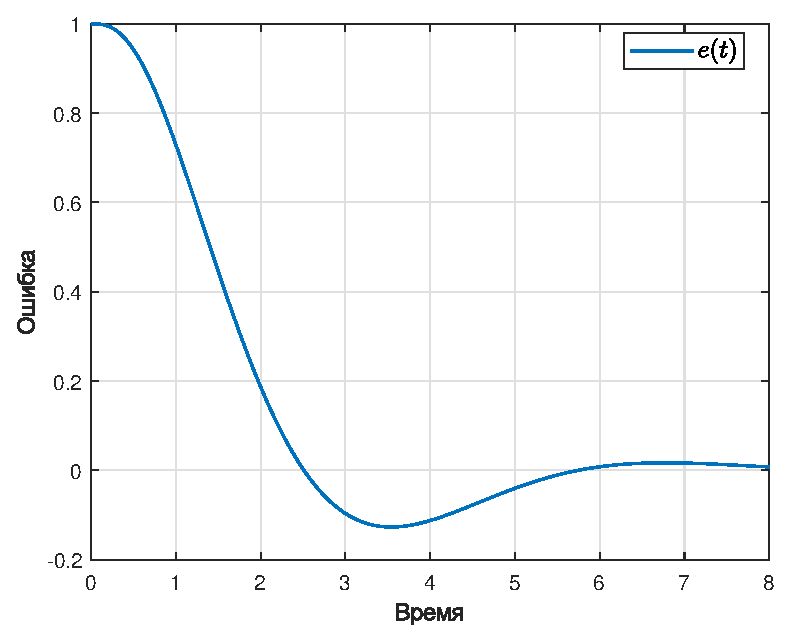
\includegraphics[width=\textwidth]{ex4/k1_g_a_error.eps}
        \caption{График ошибки при $k=1$, $g(t)=1$}
        % \centerline{лягушки}
    \end{minipage}\\[1em]
\end{figure}\noindent\

\begin{figure}[H]
    \begin{minipage}{0.5\textwidth}
        \centering 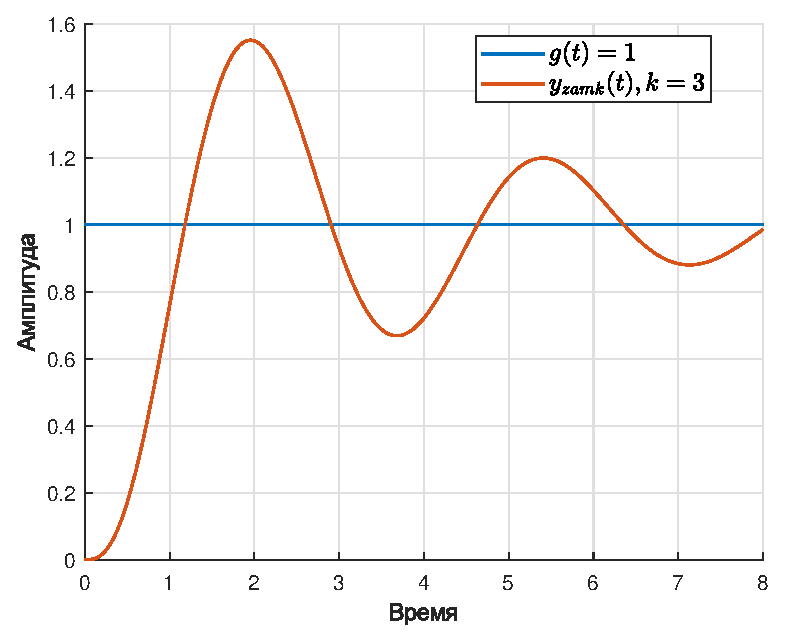
\includegraphics[width=\textwidth]{ex4/k3_g_a.eps}
        \caption{Графики входа и выхода при $k=3$, $g(t)=1$}
    \end{minipage}\hfill
    \begin{minipage}{0.5\textwidth}
        \centering 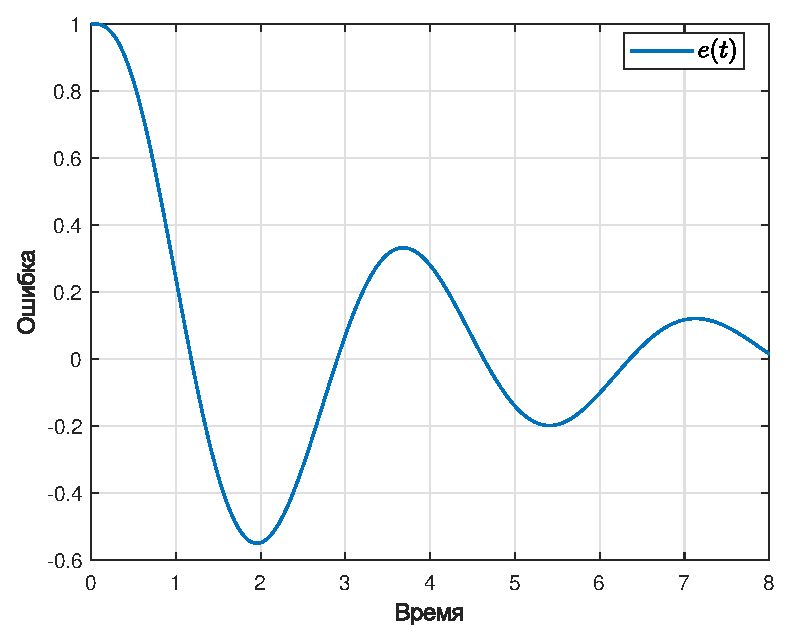
\includegraphics[width=\textwidth]{ex4/k3_g_a_error.eps}
        \caption{График ошибки при $k=3$, $g(t)=1$}
        % \centerline{лягушки}
    \end{minipage}\\[1em]
\end{figure}\noindent\

\begin{figure}[H]
    \centering
    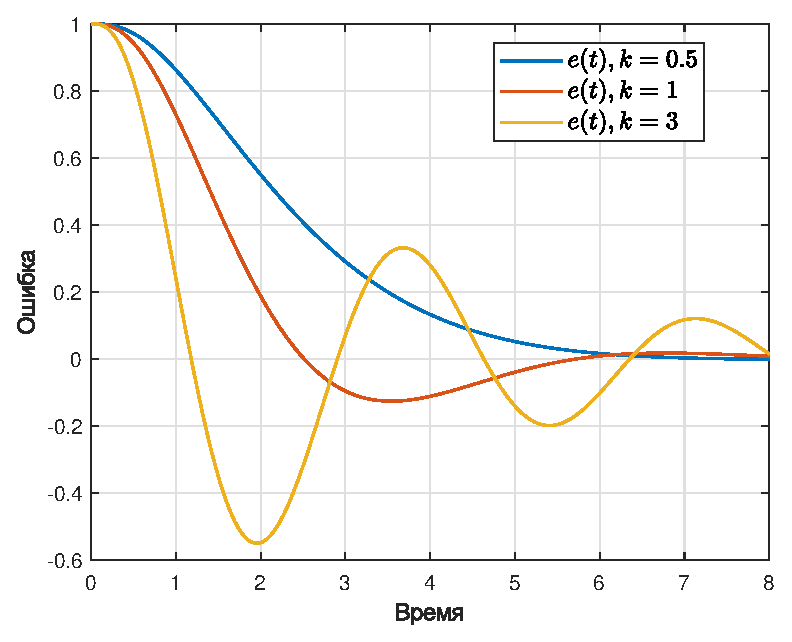
\includegraphics[width=0.55\linewidth]{ex4/all_g_a_error.eps}
    \caption{Сопоставление ошибок при $g(t)=1$}
\end{figure}\

Видим, что действительно, воздействие регулятора при всех выбранных значениях параметра $k$ делает систему астатической относительно константного воздействия --- ошибка наблюдения действительно стремится к $0$.

\subsection{Режим движения с постоянной скоростью ($g(t) = t$)}\

В этом случае ошибка не должна сойтись к 0 с течением времени, однако должна прийти к некоторому установившемуся значению, зависящему от $k$. Проверим это вычислениями:

$$
W(s) = W_{\text{s}}(s) H(s) = \frac{5k}{s(s^2+5s+6)}
$$\

$$
\underset{g\to e}{W}(s) = \frac{1}{1+W(s)} = \frac{1}{1+\frac{5k}{s(s^2+5s+6)}} = \frac{s(s^2+5s+6)}{s(s^2+5s+6) + 5k}
$$

$$
E(s) = \underset{g\to e}{W}(s) \cdot G(s) = \frac{s(s^2+5s+6)}{s(s^2+5s+6) + 5k} \cdot \frac{1}{s^2} = \frac{s(s^2+5s+6)}{s^3(s^2+5s+6) + 5ks^2}
$$

$$
e_{\text{уст}} = \lim_{t\to +\infty} e(t) = \lim_{s\to 0} sE(s) = \lim_{s\to 0} \frac{s^2(s^2+5s+6)}{s^3(s^2+5s+6) + 5ks^2} = \lim_{s\to 0} \frac{\cancelto{0}{s^2}+5\cancelto{0}{s}+6}{\cancelto{0}{s}(\cancelto{0}{s^2}+5\cancelto{0}{s}+6) + 5k} = \frac{6}{5k}.
$$\

Для $k = 0.5$ установившаяся ошибка составит $e_{\text{уст}} = \frac{6}{5\cdot 0.5} = \frac{6}{2.5}=2.4$. Для $k = 1$ --- $e_{\text{уст}} = \frac{6}{5} = 1.2$. Для $k = 3$ --- $e_{\text{уст}} = \frac{6}{5 \cdot 3} = 0.4$. Посмотрим на графики и убедимся в том, что вычисления выполнены корректно:

\begin{figure}[H]
    \begin{minipage}{0.5\textwidth}
        \centering 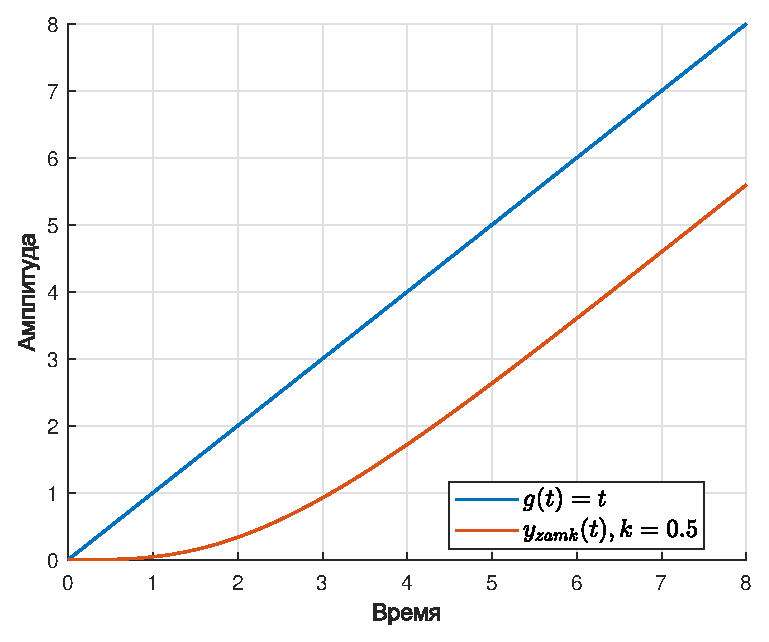
\includegraphics[width=\textwidth]{ex4/k0.5_g_vt.eps}
        \caption{Графики входа и выхода при $k=0.5$, $g(t)=t$}
    \end{minipage}\hfill
    \begin{minipage}{0.5\textwidth}
        \centering 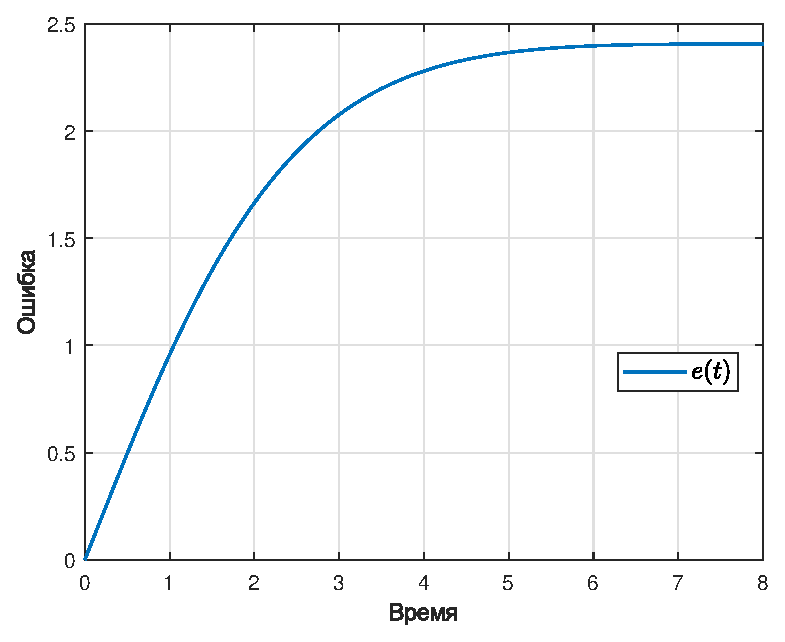
\includegraphics[width=\textwidth]{ex4/k0.5_g_vt_error.eps}
        \caption{График ошибки при $k=0.5$, $g(t)=t$}
        % \centerline{лягушки}
    \end{minipage}\\[1em]
\end{figure}\noindent\

\begin{figure}[H]
    \begin{minipage}{0.5\textwidth}
        \centering 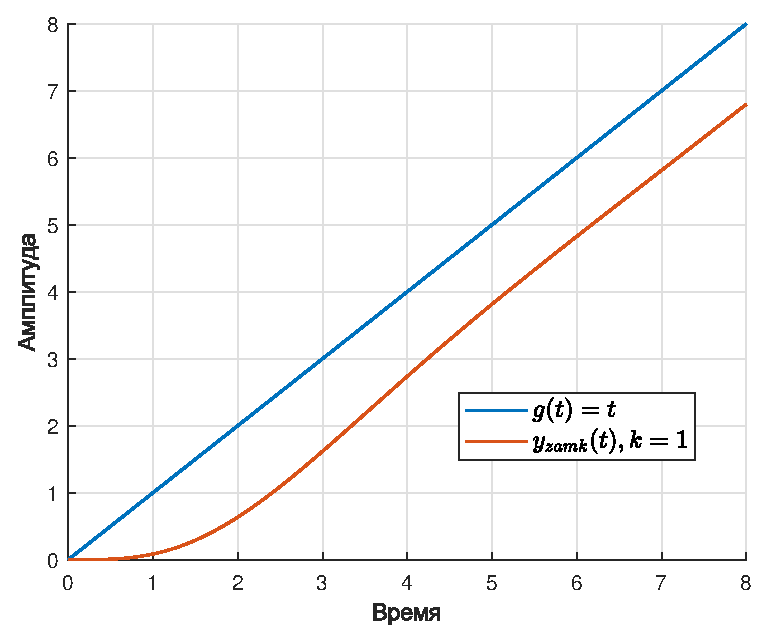
\includegraphics[width=\textwidth]{ex4/k1_g_vt.eps}
        \caption{Графики входа и выхода при $k=1$, $g(t)=t$}
    \end{minipage}\hfill
    \begin{minipage}{0.5\textwidth}
        \centering 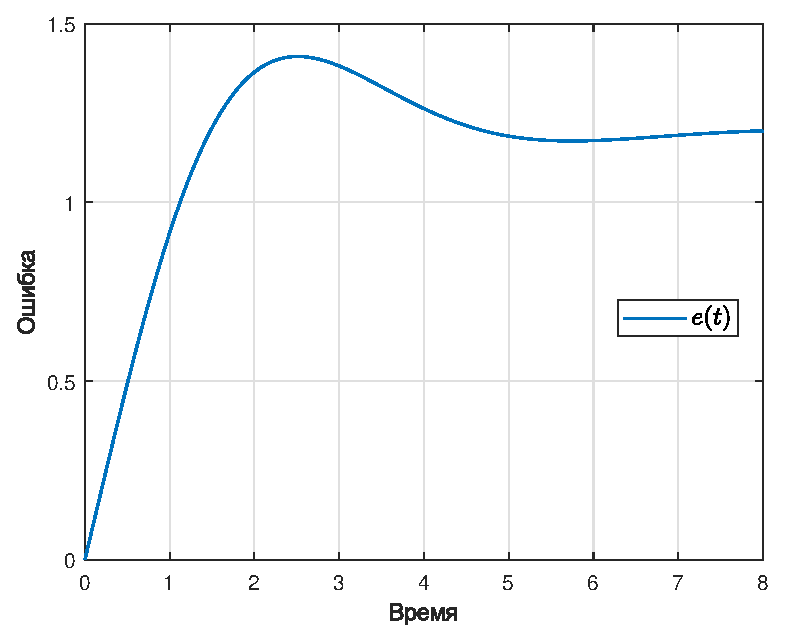
\includegraphics[width=\textwidth]{ex4/k1_g_vt_error.eps}
        \caption{График ошибки при $k=1$, $g(t)=t$}
        % \centerline{лягушки}
    \end{minipage}\\[1em]
\end{figure}\noindent\

\begin{figure}[H]
    \begin{minipage}{0.5\textwidth}
        \centering 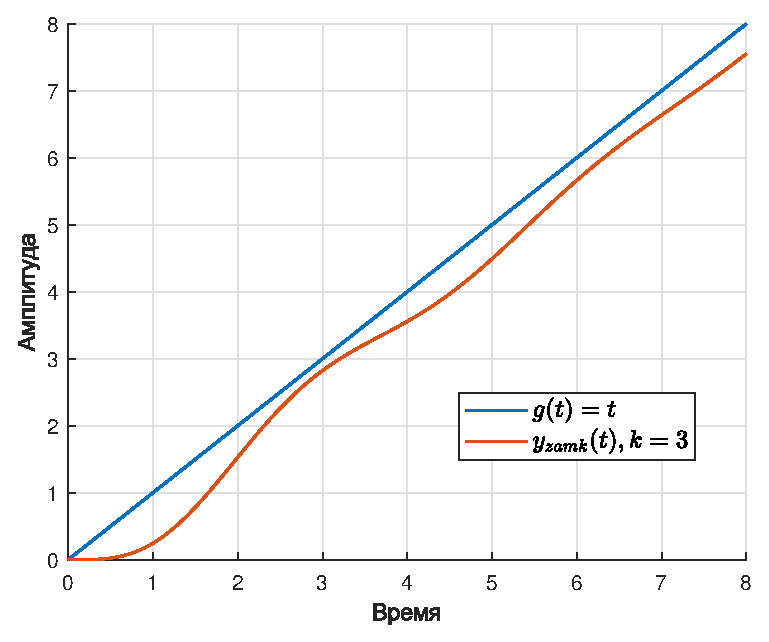
\includegraphics[width=\textwidth]{ex4/k3_g_vt.eps}
        \caption{Графики входа и выхода при $k=3$, $g(t)=t$}
    \end{minipage}\hfill
    \begin{minipage}{0.5\textwidth}
        \centering 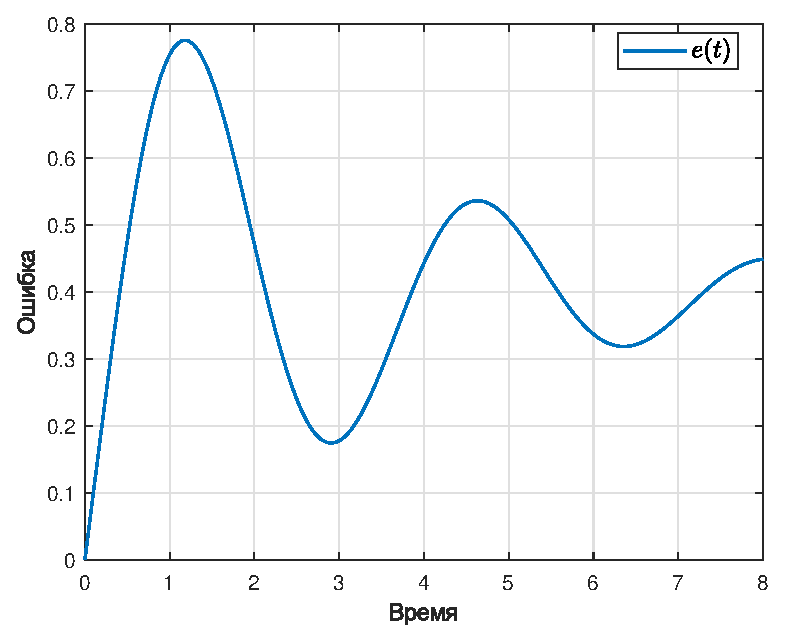
\includegraphics[width=\textwidth]{ex4/k3_g_vt_error.eps}
        \caption{График ошибки при $k=3$, $g(t)=t$}
        % \centerline{лягушки}
    \end{minipage}\\[1em]
\end{figure}\noindent\

\begin{figure}[H]
    \centering
    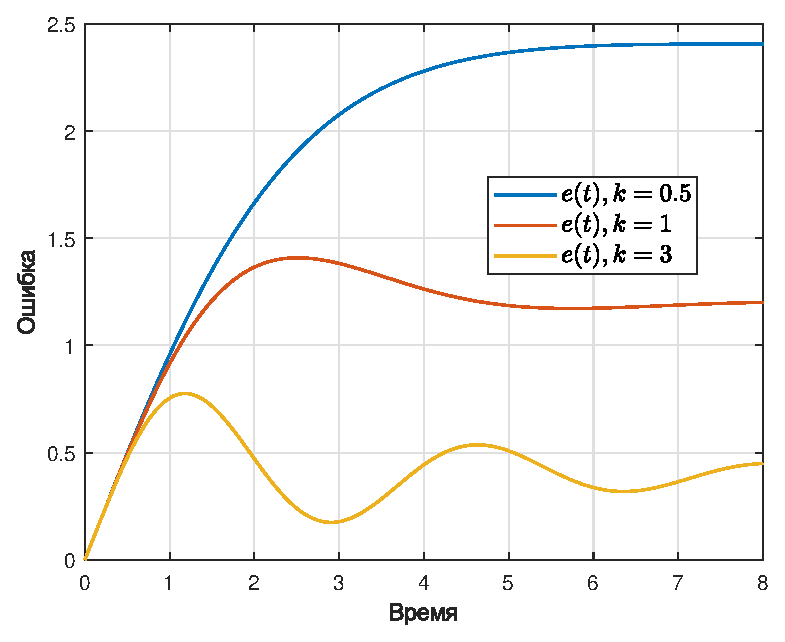
\includegraphics[width=0.55\linewidth]{ex4/all_g_vt_error.eps}
    \caption{Сопоставление ошибок при $g(t)=t$}
\end{figure}\

Видим, что снова рассчитанные аналитически установившиеся ошибки совпали с графиками. Система с И-регулятором обладает астатизмом первого порядка, что и подтверждается графиками.

\subsection{Режим движения с постоянным ускорением при $g(t) = 0.45t^2$}\

В этом случае порядок астатизма системы не позволит ей ни сойтись к постоянной ошибке наблюдения, ни, тем более, асимптотически сойтись к задающему воздействию --- $g(t)$ растёт слишком быстро.\ 

\begin{figure}[H]
    \begin{minipage}{0.5\textwidth}
        \centering 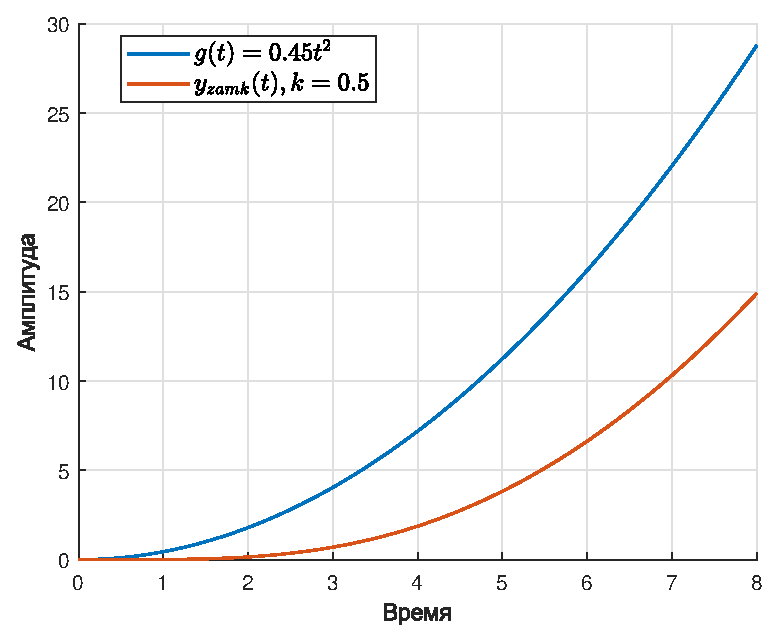
\includegraphics[width=\textwidth]{ex4/k0.5_g_at2.eps}
        \caption{Графики входа и выхода при $k=0.5$, $g(t)=0.45t^2$}
    \end{minipage}\hfill
    \begin{minipage}{0.5\textwidth}
        \centering 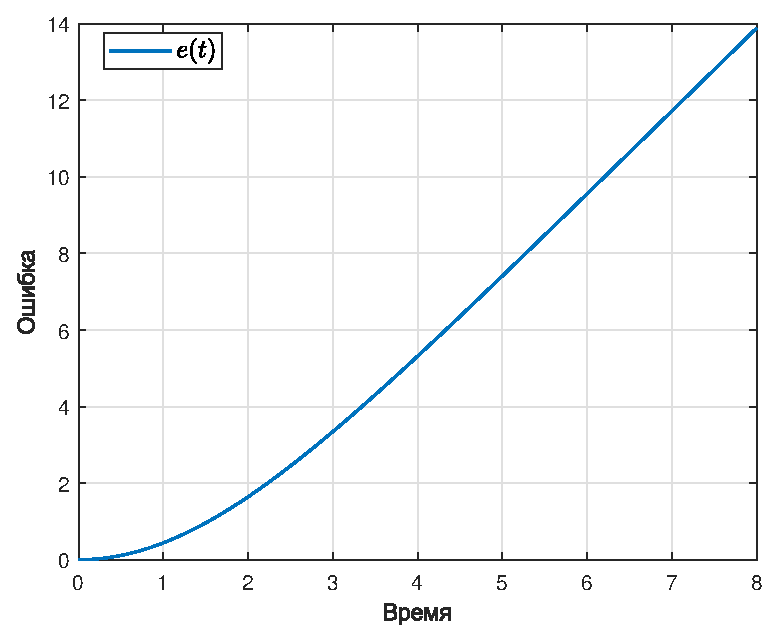
\includegraphics[width=\textwidth]{ex4/k0.5_g_at2_error.eps}
        \caption{График ошибки при $k=0.5$, $g(t)=0.45t^2$}
        % \centerline{лягушки}
    \end{minipage}\\[1em]
\end{figure}\noindent\

\begin{figure}[H]
    \begin{minipage}{0.5\textwidth}
        \centering 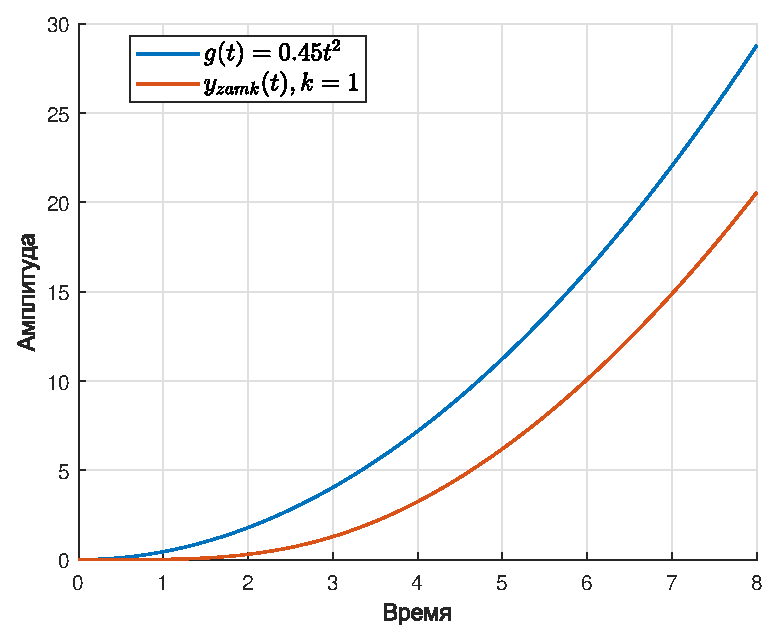
\includegraphics[width=\textwidth]{ex4/k1_g_at2.eps}
        \caption{Графики входа и выхода при $k=1$, $g(t)=0.45t^2$}
    \end{minipage}\hfill
    \begin{minipage}{0.5\textwidth}
        \centering 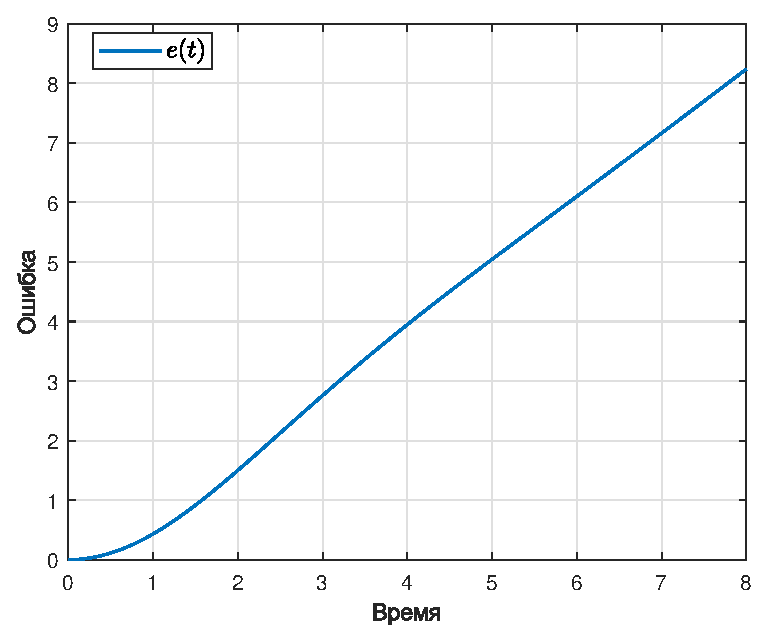
\includegraphics[width=\textwidth]{ex4/k1_g_at2_error.eps}
        \caption{График ошибки при $k=1$, $g(t)=0.45t^2$}
        % \centerline{лягушки}
    \end{minipage}\\[1em]
\end{figure}\noindent\

\begin{figure}[H]
    \begin{minipage}{0.5\textwidth}
        \centering 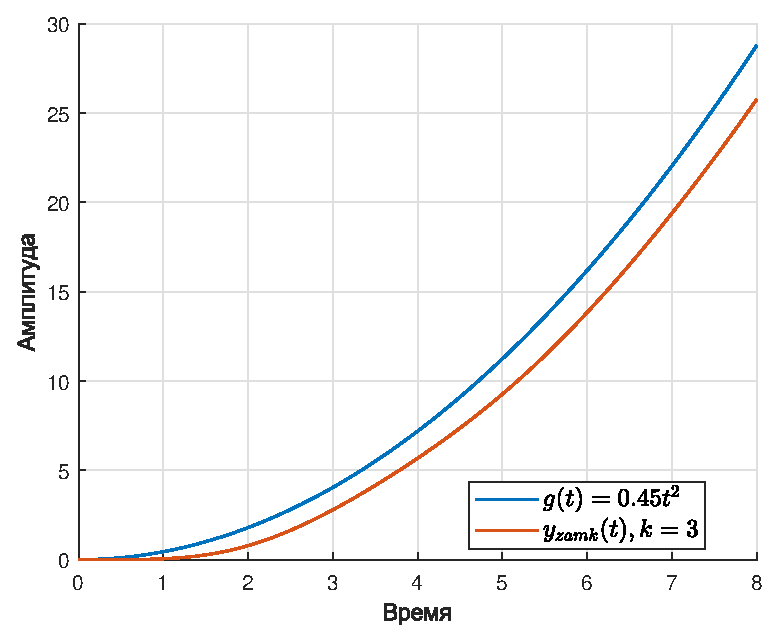
\includegraphics[width=\textwidth]{ex4/k3_g_at2.eps}
        \caption{Графики входа и выхода при $k=3$, $g(t)=0.45t^2$}
    \end{minipage}\hfill
    \begin{minipage}{0.5\textwidth}
        \centering 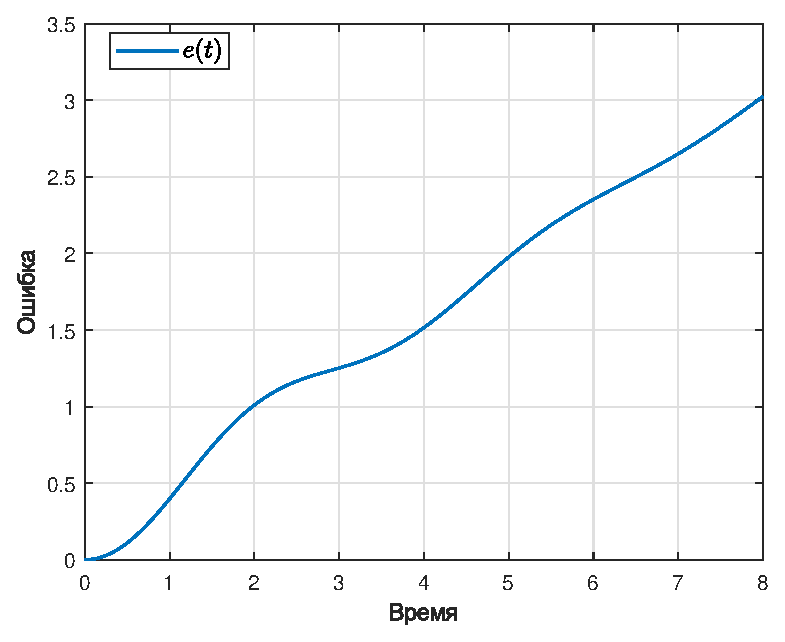
\includegraphics[width=\textwidth]{ex4/k3_g_at2_error.eps}
        \caption{График ошибки при $k=3$, $g(t)=0.45t^2$}
        % \centerline{лягушки}
    \end{minipage}\\[1em]
\end{figure}\noindent\

\begin{figure}[H]
    \centering
    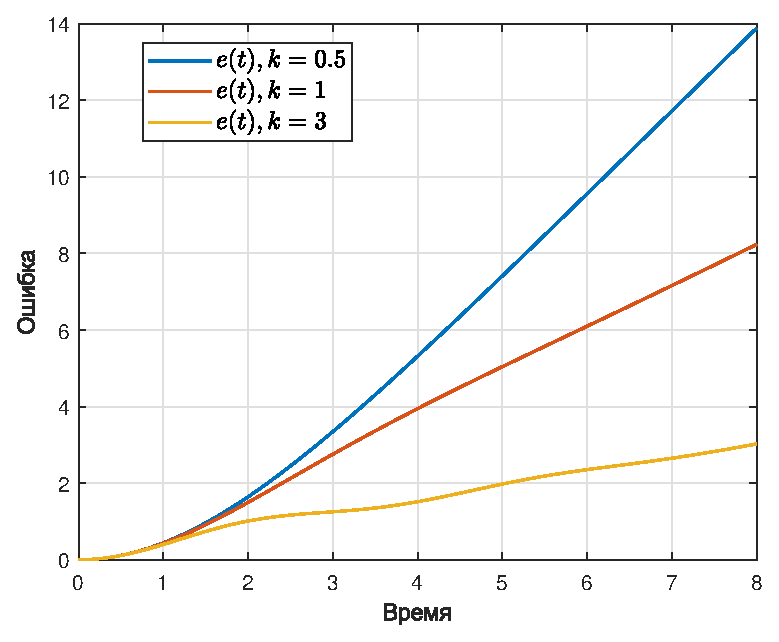
\includegraphics[width=0.55\linewidth]{ex4/all_g_at2_error.eps}
    \caption{Сопоставление ошибок при $g(t)=0.45t^2$}
\end{figure}\

Заметно, что во всех трёх случаях ошибка сходится к линейному росту, и чем больше $k$, тем больше колеблется график ошибки, и $\underset{k \to \infty}{\lim} e_{\text{уст}}(k) = 0$, но $e_{\text{уст}}$ не станет равным нулю ни при каких $k$ из-за порядка астатизма системы.

\subsection{Выводы}\ 

И-регулятор обладает большим порядком астатизма чем у П-регулятора, что позволяет ему сходиться к задающему воздействию большего порядка.

\section{Задача слежения для системы с астатизмом первого порядка (ПИ-регулятор)}\

В задании используется ПИ-регулятор $(H(s) = \frac{k_\text{И}}{s} + k_\text{П})$. Схема с его использованием представлена на рисунке:

\begin{figure}[H]
    \centering
    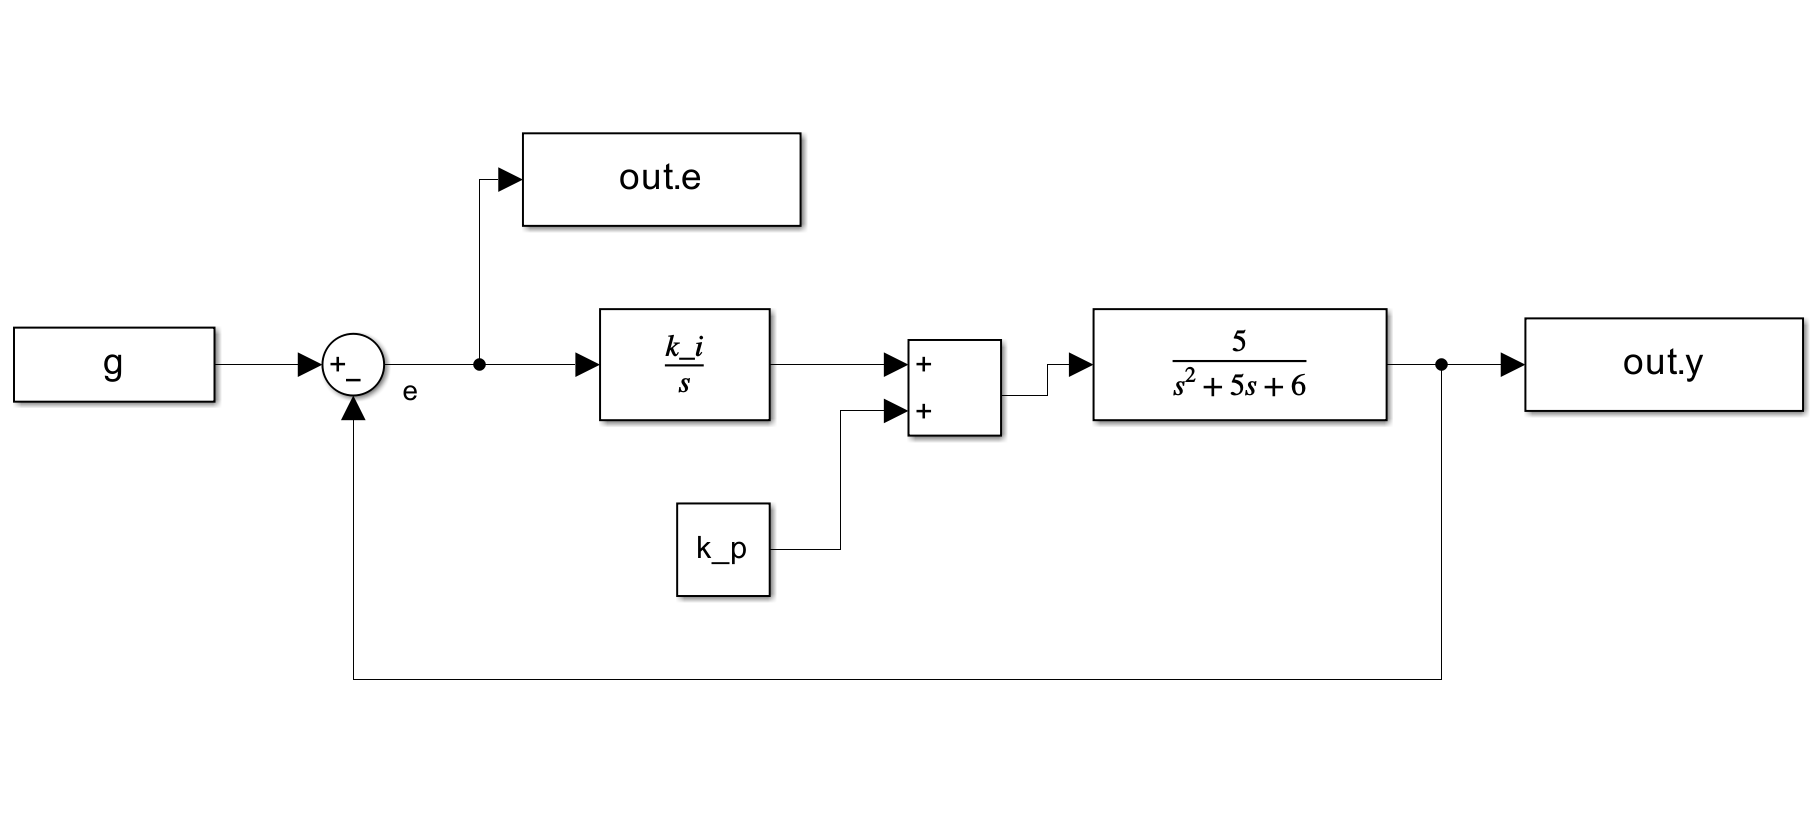
\includegraphics[width=0.65\linewidth]{ex5/scheme.png}
    \caption{Структурная схема с использованием ПИ-регулятора}
\end{figure}\

Задачу слежения буду решать, выбрав для варьирования коэффициентов  наборы $[0.3, 0.7, 1.2]$ и $[0.5, 1, 2]$ для $k_{\text{И}}$ и $k_\text{П}$ соответственно. 

\subsection{Исследование режима движения с постоянной скоростью}\

Порядок задающего воздействия на единицу больше порядка астатизма системы, значит, ошибка должна прийти к некоторому установившемуся значению, зависящему от $k$. Проверим это вычислениями:

$$
W(s) = W_{\text{s}}(s) H(s) = \frac{5}{s^2+5s+6} \cdot \left(\frac{k_\text{И}}{s} + k_\text{П}\right) = \frac{5(k_\text{П} s + k_\text{И})}{s(s^2 + 5s + 6)}
$$\

$$
\underset{g\to e}{W}(s) = \frac{1}{1+W(s)} = \frac{1}{1+\frac{5(k_\text{П} s + k_\text{И})}{s(s^2 + 5s + 6)}} = \frac{s(s^2+5s+6)}{s(s^2 + 5s + 6) + 5(k_\text{П} s + k_\text{И})}
$$

$$
E(s) = \underset{g\to e}{W}(s) \cdot G(s) = \frac{s(s^2+5s+6)}{s(s^2 + 5s + 6) + 5(k_\text{П} s + k_\text{И})} \cdot \frac{1}{s^2} = \frac{s(s^2+5s+6)}{s^3(s^2 + 5s + 6) + 5s^2(k_\text{П} s + k_\text{И})}
$$

$$
e_{\text{уст}} = \lim_{t\to +\infty} e(t) = \lim_{s\to 0} sE(s) = \lim_{s\to 0} \frac{s^2(s^2+5s+6)}{s^3(s^2 + 5s + 6) + 5s^2(k_\text{П} s + k_\text{И})} = \lim_{s\to 0} \frac{(\cancelto{0}{s^2}+\cancelto{0}{5s}+6)}{\cancelto{0}{s(s^2 + 5s + 6)} + 5(\cancelto{0}{k_\text{П} s} + k_\text{И})} = \frac{6}{5k_{\text{И}}}.
$$\

Видим, что коэффициент $k_\text{П}$ не влияет на установившуюся ошибку.\ 

В соответствии с выбранными значениями коэффициентов для $k_{\text{И}} = 0.3$ $e_{\text{уст}} = \frac{6}{5\cdot 0.3} =4$. Для $k = 0.7$ --- $e_{\text{уст}} = \frac{6}{5\cdot 0.7} \approx 1.71$. Для $k = 1.2$ --- $e_{\text{уст}} = \frac{6}{5 \cdot 1.2} = 1$. Посмотрим на графики и убедимся в том, что вычисления выполнены корректно.

\begin{figure}[H]
    \begin{minipage}{0.5\textwidth}
        \centering 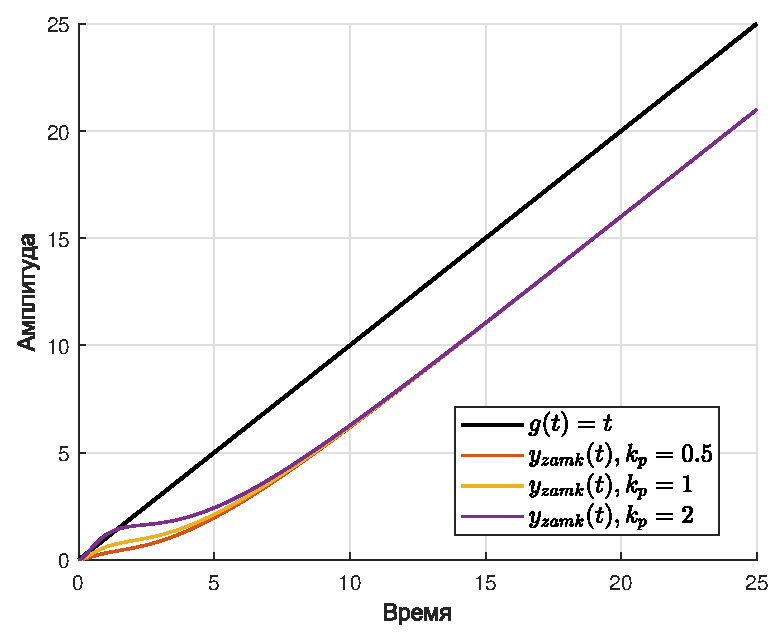
\includegraphics[width=\textwidth]{ex5/ki_0.3_g_vt.eps}
        \caption{Графики входа и выхода}
        \centerline{при $k_{\text{И}} = 0.3$, $g(t)=t$}
    \end{minipage}\hfill
    \begin{minipage}{0.5\textwidth}
        \centering 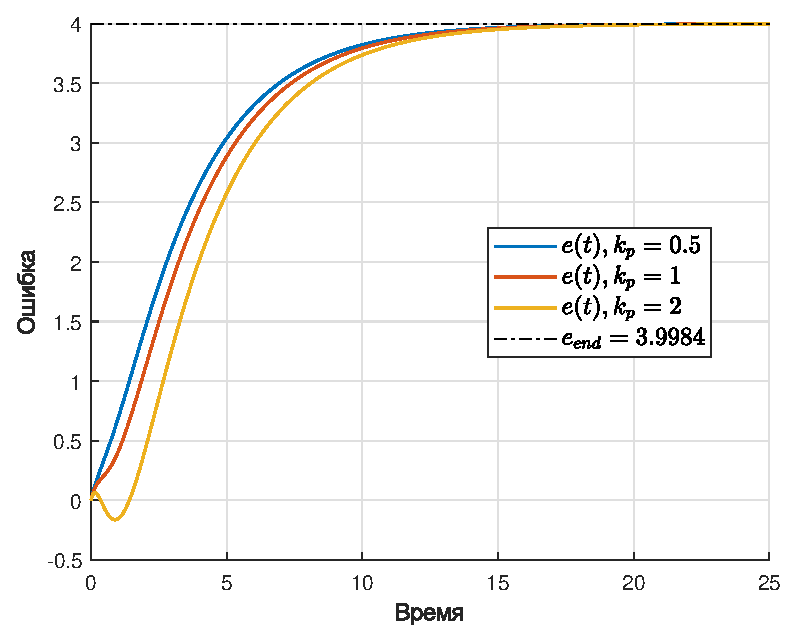
\includegraphics[width=\textwidth]{ex5/ki_0.3_g_vt_error.eps}
        \caption{График ошибки при}
        \centerline{при $k_{\text{И}} = 0.3$, $g(t)=t$}
        % \centerline{лягушки}
    \end{minipage}\\[1em]
\end{figure}\noindent\

\begin{figure}[H]
    \begin{minipage}{0.5\textwidth}
        \centering 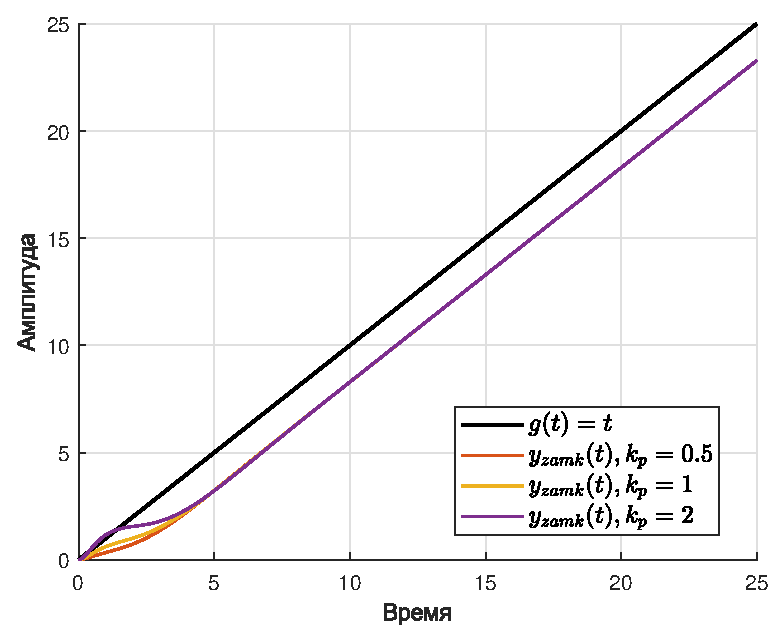
\includegraphics[width=\textwidth]{ex5/ki_0.7_g_vt.eps}
        \caption{Графики входа и выхода}
        \centerline{при $k_{\text{И}} = 0.7$, $g(t)=t$}
    \end{minipage}\hfill
    \begin{minipage}{0.5\textwidth}
        \centering 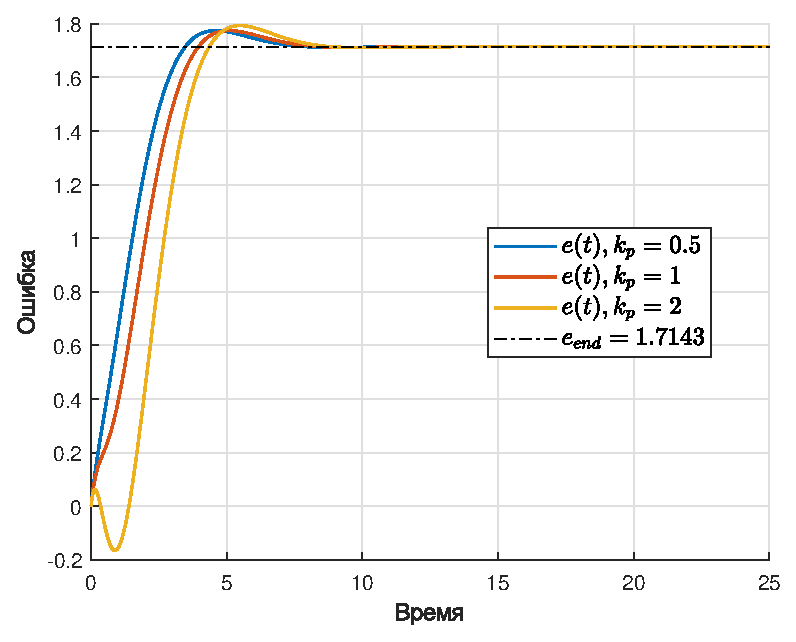
\includegraphics[width=\textwidth]{ex5/ki_0.7_g_vt_error.eps}
        \caption{График ошибки}
        \centerline{при $k_{\text{И}} = 0.7$, $g(t)=t$}
        % \centerline{лягушки}
    \end{minipage}\\[1em]
\end{figure}\noindent\

\begin{figure}[H]
    \begin{minipage}{0.5\textwidth}
        \centering 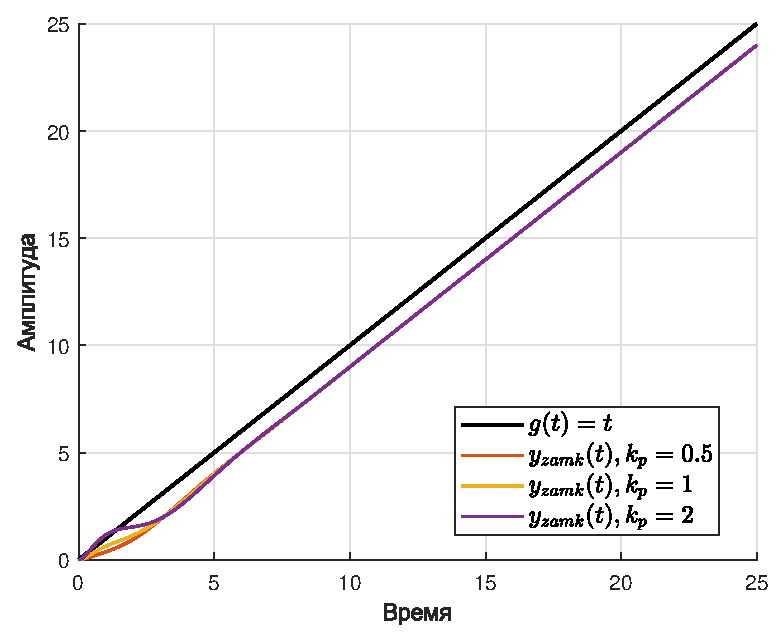
\includegraphics[width=\textwidth]{ex5/ki_1.2_g_vt.eps}
        \caption{Графики входа и выхода}
        \centerline{при $k_{\text{И}} = 1.2$, $g(t)=t$}
    \end{minipage}\hfill
    \begin{minipage}{0.5\textwidth}
        \centering 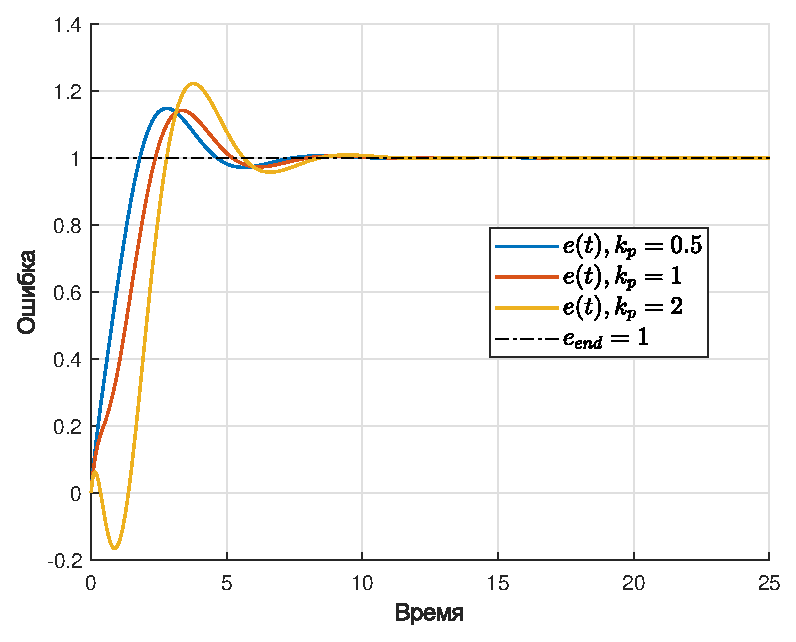
\includegraphics[width=\textwidth]{ex5/ki_1.2_g_vt_error.eps}
        \caption{График ошибки}
        \centerline{при $k_{\text{И}} = 1.2$, $g(t)=t$}
        % \centerline{лягушки}
    \end{minipage}\\[1em]
\end{figure}\noindent\

На всех рассмотренных наборах значений коэффициентов $k_{\text{И}}$, $k_{\text{П}}$ аналитические расчёты установившейся ошибки совпадают с моделированием. Также можно сделать выводы о влиянии пропорционального коэффициента $k_{\text{П}}$ и интегрального коэффициента $k_{\text{И}}$ на поведение системы --- чем выше значение интегрального коэффициента, тем быстрее система сходится к установившемуся значению ошибки, и тем сильнее приближается к задающему воздействию. Увеличение $k_{\text{П}}$ также ускоряет реакцию системы (уменьшает время переходного процесса) и приводит к увеличению колебательности системы (как и увеличение $k_{\text{И}}$), и наоборот. То есть если стоит задача минимизации ошибки наблюдения, то максимально повышаем $k_{\text{И}}$, и подбираем значение $k_{\text{П}}$ для уменьшения избыточного перерегулирования так, чтобы система оставалась устойчивой.


\subsection{Исследование режима слежения за гармоническим сигналом}\

Теперь в качестве задающего воздействия будет использоваться $g(t) = \sin{(0.45t)} \Rightarrow G(s) = \frac{0.45}{0.45^2 + s^2}$.\

В этом случае ошибка не будет постоянной, и нельзя найти её установившееся значение. Промоделируем схему с соответствующим заданию гармоническим сигналом $g(t) = \sin{(0.45t)}$:

\begin{figure}[H]
    \begin{minipage}{0.5\textwidth}
        \centering 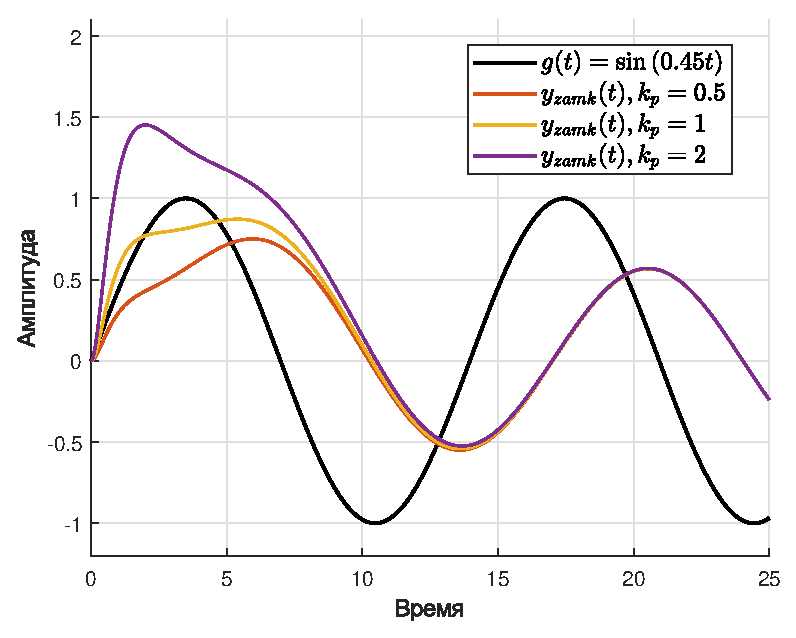
\includegraphics[width=\textwidth]{ex5/ki_0.3_g_asinwt.eps}
        \caption{Графики входа и выхода}
        \centerline{при $k_{\text{И}} = 0.3$, $g(t) = \sin{(0.45t)}$}
    \end{minipage}\hfill
    \begin{minipage}{0.5\textwidth}
        \centering \includegraphics[width=\textwidth]{ex5/ki_0.3_g_asinwt_error.eps}
        \caption{График ошибки}
        \centerline{при $k_{\text{И}} = 0.3$, $g(t) = \sin{(0.45t)}$}
    \end{minipage}\\[1em]
\end{figure}\noindent\

\begin{figure}[H]
    \begin{minipage}{0.5\textwidth}
        \centering \includegraphics[width=\textwidth]{ex5/ki_0.7_g_asinwt.eps}
        \caption{Графики входа и выхода}
        \centerline{при $k_{\text{И}} = 0.7$, $g(t) = \sin{(0.45t)}$}
    \end{minipage}\hfill
    \begin{minipage}{0.5\textwidth}
        \centering \includegraphics[width=\textwidth]{ex5/ki_0.7_g_asinwt_error.eps}
        \caption{График ошибки}
        \centerline{при $k_{\text{И}} = 0.7$, $g(t) = \sin{(0.45t)}$}
    \end{minipage}\\[1em]
\end{figure}\noindent\

\begin{figure}[H]
    \begin{minipage}{0.5\textwidth}
        \centering \includegraphics[width=\textwidth]{ex5/ki_1.2_g_asinwt.eps}
        \caption{Графики входа и выхода}
        \centerline{при $k_{\text{И}} = 1.2$, $g(t) = \sin{(0.45t)}$}
    \end{minipage}\hfill
    \begin{minipage}{0.5\textwidth}
        \centering \includegraphics[width=\textwidth]{ex5/ki_1.2_g_asinwt_error.eps}
        \caption{График ошибки}
        \centerline{при $k_{\text{И}} = 1.2$, $g(t) = \sin{(0.45t)}$}
    \end{minipage}\\[1em]
\end{figure}\noindent\

Заметно уменьшение амплитуды гармонической ошибки при увеличении $k_{\text{И}}$ и увеличение колебаний в начале движения при увеличении $k_{\text{П}}$. График ошибки не сходится к прямой из-за гармонического задающего сигнала. Для достижения ошибки, сходящейся к константному значению требуется повысить порядок астатизма системы заменой регулятора.

\subsection{Выводы}\

В результате выполнения задания удалось проследить за линейно растущим входным сигналом с установившейся ошибкой, что подтверждает теоретические выкладки о поведении систем с первым порядком астатизма, рассмотренные на лекции. Если повысить порядок астатизма на 1, удастся свести ошибку наблюдения к нулю в случае линейно растущего задающего воздействия. 

\section{Задача слежения за гармоническим сигналом (регулятор общего вида)}\

В задании рассматривается регулятор общего вида, заданный передаточной функцией

$$
H(s) = \frac{\sum_{k=0}^{m}b_ks_k}{\sum_{k=0}^{m}a_ks_k}.
$$\

В качестве задаюшего воздействия в систему подаётся $g(t) = \sin{(0.45t)} \Rightarrow G(s) = \frac{0.45}{0.45^2 + s^2}$. Задача --- синтезировать регулятор. Для её решения найдём передаточную функцию по ошибке, приняв $H(s) = \frac{R(s)}{Q(s)}$. 

$$\underset{g\to e}{W}(s) = \frac{1}{1+W_s(s)H(s)} = \frac{1}{1+\frac{5}{s^2+5s+6}\frac{R(s)}{Q(s)}} = \frac{(s^2+5s+6)Q(s)}{(s^2+5s+6)Q(s)+5R(s)}$$\

Попробуем применить теорему о предельном значении:

$$e_{\text{уст}} = \lim_{t\to +\infty} e(t) = \lim_{s\to 0} s\underset{g\to e}{W}(s) G(s) = \lim_{s\to 0}\frac{0.45(s^2+5s+6)Q(s)}{(0.45^2 + s^2)((s^2+5s+6)Q(s)+5R(s))}$$\

Видим, что теорема не применима из-за множителя $(0.45^2 + s^2)$ в знаменателе, имеющего положительный корень. Введём $Q(s) = Q'(s)(0.45^2 + s^2)$, тогда уравнение примет следующий вид:

$$\lim_{s\to 0}\frac{0.45(s^2+5s+6)Q'(s)\cancel{(0.45^2 + s^2)}}{((s^2+5s+6)Q'(s)(0.45^2 + s^2)+5R(s))\cancel{(0.45^2 + s^2)}} = \lim_{s\to 0}\frac{0.45(s^2+5s+6)Q'(s)}{((s^2+5s+6)Q'(s)(0.45^2 + s^2)+5R(s))}$$.\

Система асимптотически устойчива, если все полюса знаменателя дроби в пределе отрицательны. Пусть $Q'(s) = a_3s + a_2$. Тогда $Q(s) = (0.45^2 + s^2)(a_3s + a_2)$. Примем $R(s)$ того же порядка, что и $Q(s)$: $R(s) = b_3s^3 + b_2s^2+b_1s + b_0$. Тогда знаменатель:

$$(s^2+5s+6)Q'(s)(0.45^2 + s^2)+5R(s) = $$
$$=(s^2 + 5s + 6)(s^2 + 0.45^2)(a_3 s + a_2) + 5(b_3 s^3 + b_2 s^2 + b_1 s + b_0).$$\
$$(s^2 + 5s + 6)(s^2 + 0.45^2)= s^2(s^2 + 0.45^2) + 5s(s^2 + 0.45^2) + 6(s^2 + 0.45^2) = s^4 + 5s^3 + (0.45^2 + 6)s^2 + 5\cdot0.45^2 s + 6\cdot0.45^2.$$\
$$(s^2 + 5s + 6)(s^2 + 0.45^2)(a_3s + a_2)=$$
$$= a_3(s^5 + 5s^4 + (0.45^2 + 6) s^3 + 5\cdot0.45^2 s^2 + 6\cdot0.45^2 s) + a_2(s^4 + 5s^3 + (0.45^2 + 6) s^2 + 5\cdot0.45^2 s + 6\cdot0.45^2)=$$
$$=a_3 s^5 + (5a_3 + a_2)s^4 + ((0.45^2 + 6) a_3 + 5a_2)s^3 + (5\cdot0.45^2 a_3 + (0.45^2 + 6) a_2)s^2 + (6\cdot0.45^2 a_3 + 5\cdot0.45^2 a_2)s + 6\cdot0.45^2 a_2.$$\

Получили полином $C(s) = c_5s^5 + c_4s^4+c_3s^3+c_2s^2+c_1s + c_0$, где $c_5 = a_3, c_4 = 5a_3 + a_2, c_3 = (0.45^2 + 6) a_3 + 5a_2 + 5b_3, c_2 = 5\cdot0.45^2 a_3 + (0.45^2 + 6) a_2 + 5b_2, c_1 = 6\cdot0.45^2 a_3 + 5\cdot0.45^2 a_2 + 5b_1, c_0 = (0.45^2 + 6) a_2 + 5b_0.$\ Вычислим для него конкретные параметры $c_i$, воспользовавшись типовым полиномом Баттерворта с коэффициентом подобия $\omega_0 = 1$. Полином Баттерворта пятой степени:

$$
s^5 + 3.24\omega_0s^4+15.24\omega_0^2s^3+15.24\omega_0^3s^2+3.24\omega_0^4s + \omega^5
$$\

При коэффициенте подобия $\omega_0 = 1$:

$$
s^5 + 3.24s^4+15.24s^3+15.24s^2+3.24s + 1
$$

Сопоставим коэффициенты при равных степенях этого полинома и $C(s)$:

$$
\begin{cases}
    a_3 = 1, \\
    5a_3 + a_2 = 3.24, \\ 
    (0.45^2 + 6) a_3 + 5a_2 + 5b_3 = 15.24, \\
    0.45^2 \cdot 5 a_3 + (0.45^2 + 6) a_2 + 5b_2 = 15.24, \\
    0.45^2 \cdot 6 a_3 + 0.45^2 \cdot 5 a_2 + 5b_1 = 3.24, \\
    0.45^2 \cdot 6 a_2 + 5b_0 = 1.
\end{cases} \Leftrightarrow \begin{cases}
    a_3 = 1, \\
    a_2 = -1.76, \\ 
    b_3 = 1.57, \\
    b_2 = 3.03, \\
    b_1 = 0.76, \\
    b_0 = 0.62.
\end{cases}
$$

Тогда образ Лапласа регулятора выглядит следующим образом:

$$
H(s) = \frac{R(s)}{Q(s)} = \frac{b_3s^3+b_2s^2 + b_1s + b_0}{a_3s^3 + a_2s^2 + a_1 s + a_0}.
$$\ 

Также вспомним, что

$$Q(s) = Q'(s)(0.45^2+s^2) = (a_3s + a_2)(0.45^2+s^2) = a_3s^3 + a_2 s^2 + 0.45^2a_3s + 0.45^2a_2.$$

Подставляя найденные значения коэффициентов, получаем

$$
H(s) = \frac{1.57s^3 + 3.03s^2 + 0.76s + 0.62}{s^3-1.76s^2+0.2025s-0.3564}.
$$\ 

Проверим работоспособность синтезированного регулятора, найдя его установившуюся ошибку:


$$\underset{g\to e}{W}(s) = \frac{1}{1+W_s(s)H(s)} = \frac{1}{1+\frac{5}{s^2+5s+6}\frac{1.57s^3 + 3.03s^2 + 0.76s + 0.62}{s^3-1.76s^2+0.2025s-0.3564}}=$$

$$ = \frac{(s^3-1.76s^2+0.2025s-0.3564)(s^2+5s+6)}{(s^3-1.76s^2+0.2025s-0.3564)(s^2+5s+6) + 5(1.57s^3 + 3.03s^2 + 0.76s + 0.62)}$$

$$
e_{\text{уст}} = \lim_{t\to +\infty} e(t) = \lim_{s\to 0} s\underset{g\to e}{W}(s) G(s) =
$$

$$
= \lim_{s\to 0}\frac{0.45s(s^3-1.76s^2+0.2025s-0.3564)(s^2+5s+6)}{(s^3-1.76s^2+0.2025s-0.3564)(s^2+5s+6) + 5(1.57s^3 + 3.03s^2 + 0.76s + 0.62)(0.45^2 + s^2)}=
$$

$$
= \frac{0}{-0.3654\cdot6\cdot5\cdot0.62\cdot0.45^2} = 0
$$\ 

Теоретически устойчивость синтезированного регулятора подтверждается. Теперь время провести реальное моделирование:

\begin{figure}[H]
    \begin{minipage}{0.5\textwidth}
        \centering \includegraphics[width=\textwidth]{ex6/sin.eps}
        \caption{Графики входа и выхода}
    \end{minipage}\hfill
    \begin{minipage}{0.5\textwidth}
        \centering \includegraphics[width=\textwidth]{ex6/error_0.135.eps}
        \caption{График ошибки}
    \end{minipage}\\[1em]
\end{figure}\noindent\

Судя по графику, время переходного процесса составило $7.99$ секунд. Так как выбрано $\omega_0 = 1$, то по теореме подобия это время должно соответствовать данному в таблице из материалов практики для 5-го порядка системы ($7.7$). Значения совпадают неидельно.

\subsection{Выводы}\

В задании был синтезирован регулятор, следящий за гармоническим сигналом, проверена его работоспособность. Действия, осуществленные для синтезирования конкретно этого регулятора, по сути совпадают с действиями, необходимыми для синтезирования и других регуляторов. Так что можно заключить, что выполнив задание, я научился синтезировать регуляторы.

\section{Вывод по работе}\ 

Выполнив лабораторную работу, я познакомился с задачами стабилизации и слежения, а также с их решениями, посмотрел на простейшие виды регуляторов, выявил связь между ``подвижностью'' системы и порядком астатизма, научился понимать, какой вид сигнала система может отследить с нулевой установившейся ошибкой, научился аналитически выводить статическую ошибку от внешнего воздействия по передаточным функциям, осознал как синтезировать регуляторы 

\section{Приложение А. Код для выполнения заданий}

\subsection*{Листинг 1. Код для выполнения задания 1}

\begin{lstlisting}[caption={Код для построения графиков для задания 1}, language=matlab]
% clear all;
close all;

[~, scriptName] = fileparts(mfilename('fullpath'));
if ~isfolder(scriptName)
    mkdir(scriptName);
end

t = (0:0.01:8)';
% u = [t, 1.5*ones(size(t))];
% u = [t, 0.6*t];
u = [t, zeros(size(t))];

fig_svob = figure;
out = sim('ex1/model.slx','StopTime','8');
y_model = out.y;
plot(y_model.Time, y_model.Data, LineWidth=1.2, DisplayName="$y_{raz}(t)$")
xlabel('Время'), ylabel('Амплитуда')
grid on
legend(Interpreter='latex', Location='best', BackgroundAlpha=.1, FontSize=12, FontName='Computer Modern')
saveas(fig_svob, string(scriptName) + '\' + 'razomk_fig' + '.eps', 'epsc')

k0 = 1;
k1 = 3; % траектория становится ограниченной при k1 = 1, k1 > 1 - система Ау, k1 < 1 - Ну

fig_regulator = figure;
out = sim('ex1/model_regulator.slx','StopTime','8');
y_model = out.y;
plot(y_model.Time, y_model.Data, LineWidth=1.2, DisplayName="$y_{zamk}(t)$")
xlabel('Время'), ylabel('Амплитуда')
grid on
legend(Interpreter='latex', Location='best', BackgroundAlpha=.1, FontSize=12, FontName='Computer Modern')
saveas(fig_regulator, string(scriptName) + '\' + 'zamk_fig' + '.eps', 'epsc')


% figure;
% num = [1];
% den = [1 -4 5];
% sys = tf(num, den);
% y = lsim(sys, u(:,2), t);
% plot(t, y)
\end{lstlisting}
\subsection*{Листинг 2. Код для выполнения задания 2}

\begin{lstlisting}[caption={Код для построения графиков для задания 2}, language=matlab]
% clear all;
close all;

[~, scriptName] = fileparts(mfilename('fullpath'));
if ~isfolder(scriptName)
    mkdir(scriptName);
end

t = (0:0.01:8)';
% u = [t, 1.5*ones(size(t))];
% u = [t, 0.6*t];
u = [t, zeros(size(t))];

T = 0.01;

k0 = 1;
k1 = 3; % траектория становится ограниченной при k1 = 1, k1 > 1 - система Ау, k1 < 1 - Ну

fig_regulator = figure;
hold on; grid on;

out = sim('ex1/model_regulator.slx','StopTime','8');
y_model = out.y;
plot(y_model.Time, y_model.Data, LineWidth=1.5, DisplayName="$y_{zamk}(t)$", Color='black')

out = sim('ex2/model_regulator2.slx','StopTime','8');
y_model = out.y;
plot(y_model.Time, y_model.Data, LineWidth=1.3, DisplayName="$y_{z}(t), T = " + string(T) + "$")
T = 0.4;

out = sim('ex2/model_regulator2.slx','StopTime','8');
y_model = out.y;
plot(y_model.Time, y_model.Data, LineWidth=1.3, DisplayName="$y_{z}(t), T = " + string(T) + "$")

T = 0.2;
out = sim('ex2/model_regulator2.slx','StopTime','8');
y_model = out.y;
plot(y_model.Time, y_model.Data, LineWidth=1.3, DisplayName="$y_{z}(t), T = " + string(T) + "$")

T = 0.1;
out = sim('ex2/model_regulator2.slx','StopTime','8');
y_model = out.y;
plot(y_model.Time, y_model.Data, LineWidth=1.3, DisplayName="$y_{z}(t), T = " + string(T) + "$")

xlabel('Время'), ylabel('Амплитуда')
ylim([-2, 3])
legend(Interpreter='latex', Location='best', BackgroundAlpha=.3, FontSize=12, FontName='Computer Modern')
saveas(fig_regulator, string(scriptName) + '\' + string(T) + '.eps', 'epsc')
\end{lstlisting}


\subsection*{Листинг 3. Код для выполнения задания 3}
\begin{lstlisting}[caption={Код для построения графиков для задания 3}, language=matlab]
% clear all;
close all;

[~, scriptName] = fileparts(mfilename('fullpath'));
if ~isfolder(scriptName)
    mkdir(scriptName);
end

t = (0:0.01:8)';

% g_strs = {'g_a', 'g_vt', 'g_at2', 'g_asinwt'};
g_strs = {'g_a', 'g_vt'};
g_latexs = {'1', 't', '0.45t^2', '\sin{(0.45 t)}'};
g_variants = [ones(size(t)), t, 0.45.*t.^2, sin(0.45.*t)];

for i = 1:numel(g_strs)
    g = [t, g_variants(:, i)];
    g_str = g_strs{i};
    g_latex = g_latexs{i};
    for k = [100]
        fig_regulator = figure;
        hold on; grid on;

        out = sim('ex3/model_regulator3.slx','StopTime','8');
        y_model = out.y;
        error = out.e;
        plot(t, g(:,2), LineWidth=1.2, DisplayName="$g(t) = " + g_latex + "$")
        plot(y_model.Time, y_model.Data, LineWidth=1.2, DisplayName="$y_{zamk}(t), k = " + string(k) + "$")
        xlabel('Время'), ylabel('Амплитуда')
        legend(Interpreter='latex', Location='best', BackgroundAlpha=.3, FontSize=12, FontName='Computer Modern')

        fig_error = figure;
        plot(error.Time, error.Data, LineWidth=1.2, DisplayName="$e(t)$")
        grid on;
        legend(Interpreter='latex', Location='best', BackgroundAlpha=.3, FontSize=12, FontName='Computer Modern')
        xlabel('Время'), ylabel('Ошибка')
        saveas(fig_regulator, string(scriptName) + '\k' + string(k) + '_' + g_str + '.eps', 'epsc')
        saveas(fig_error, string(scriptName) + '\k' + string(k) + '_' + g_str + '_error.eps', 'epsc')
    end
end
\end{lstlisting}

\subsection*{Листинг 4. Код для выполнения задания 4}
\begin{lstlisting}[caption={Код для построения графиков для задания 4}, language=matlab]
% clear all;
close all;

[~, scriptName] = fileparts(mfilename('fullpath'));
if ~isfolder(scriptName)
    mkdir(scriptName);
end

t = (0:0.01:8)';

% g_strs = {'g_a', 'g_vt', 'g_at2', 'g_asinwt'};
g_strs = {'g_a', 'g_vt', 'g_at2'};
g_latexs = {'1', 't', '0.45t^2', '\sin{(0.45 t)}'};
g_variants = [ones(size(t)), t, 0.45.*t.^2, sin(0.45.*t)];

for i = 1:numel(g_strs)
    g = [t, g_variants(:, i)];
    g_str = g_strs{i};
    g_latex = g_latexs{i};
    for k = [0.5, 1, 3]
        fig_regulator = figure;
        hold on; grid on;

        out = sim('ex4/model_regulator4.slx','StopTime','8');
        y_model = out.y;
        error = out.e;
        plot(t, g(:,2), LineWidth=1.2, DisplayName="$g(t) = " + g_latex + "$")
        plot(y_model.Time, y_model.Data, LineWidth=1.2, DisplayName="$y_{zamk}(t), k = " + string(k) + "$")
        xlabel('Время'), ylabel('Амплитуда')
        legend(Interpreter='latex', Location='best', BackgroundAlpha=.3, FontSize=12, FontName='Computer Modern')

        fig_error = figure;
        plot(error.Time, error.Data, LineWidth=1.2, DisplayName="$e(t)$")
        grid on; hold on;
        if (i == 2)
            e_steady = error.Data(end);
            xl = xlim;                     % текущие пределы по X - вектор [x_min, x_max]
            plot(xl, [e_steady, e_steady], 'k-.', Color='black', DisplayName="$e_{end} = " + string(e_steady) + "$");     % два значения y0 для двух точек
        end
        legend(Interpreter='latex', Location='best', BackgroundAlpha=.3, FontSize=12, FontName='Computer Modern')
        xlabel('Время'), ylabel('Ошибка')
        saveas(fig_regulator, string(scriptName) + '\k' + string(k) + '_' + g_str + '.eps', 'epsc')
        saveas(fig_error, string(scriptName) + '\k' + string(k) + '_' + g_str + '_error.eps', 'epsc')
    end
end
\end{lstlisting}

\subsection*{Листинг 5. Код для выполнения задания 5}
\begin{lstlisting}[caption={Код для построения графиков для задания 5}, language=matlab]
% clear all;
close all;

[~, scriptName] = fileparts(mfilename('fullpath'));
if ~isfolder(scriptName)
    mkdir(scriptName);
end

t = (0:0.01:25)';

% g_strs = {'g_a', 'g_vt', 'g_at2', 'g_asinwt'};
g_strs = {'g_vt', 'g_asinwt'};
g_latexs = {'t', '\sin{(0.45 t)}'};
g_variants = [t, sin(0.45.*t)];

for i = 1:numel(g_strs)
    g = [t, g_variants(:, i)];
    g_str = g_strs{i};
    g_latex = g_latexs{i};
    for k_i = [0.3, 0.7, 1.2]
        fig_regulator = figure;
        ax_regulator = gca;
        fig_error = figure;
        ax_error = gca;
        xlabel(ax_regulator, 'Время'), ylabel(ax_regulator, 'Амплитуда')
        xlabel(ax_error, 'Время'), ylabel(ax_error, 'Ошибка')
        hold(ax_regulator, 'on'); grid(ax_regulator, 'on');
        hold(ax_error, 'on'); grid(ax_error, 'on');
        plot(ax_regulator, t, g(:,2), LineWidth=1.5, DisplayName="$g(t) = " + g_latex + "$", Color='black')
        for k_p = [0.5, 1, 2]
            out = sim('ex5/model_regulator5.slx','StopTime','25');
            y_model = out.y;
            error = out.e;
            plot(ax_regulator, y_model.Time, y_model.Data, LineWidth=1.2, DisplayName="$y_{zamk}(t), k_p = " + string(k_p) + "$")
            legend(Interpreter='latex', Location='best', BackgroundAlpha=.3, FontSize=10, FontName='Computer Modern')
            plot(ax_error, error.Time, error.Data, LineWidth=1.2, DisplayName="$e(t), k_p = " + string(k_p) + "$")
        end
        if (i == 1)
            e_steady = error.Data(end);
            xl = xlim(ax_error);                     % текущие пределы по X - вектор [x_min, x_max]
            plot(ax_error, xl, [e_steady, e_steady], 'k-.', Color='black', DisplayName="$e_{end} = " + string(e_steady) + "$");     % два значения y0 для двух точек
        end
        if (i == 2)
            ylim(ax_regulator, [-1.2, 2.1])
        end
        % xlim(ax_error, [0, 25]); xlim(ax_regulator, [0, 25]); 
        legend(ax_regulator, Interpreter='latex', Location='best', BackgroundAlpha=.3, FontSize=12, FontName='Computer Modern')
        legend(ax_error, Interpreter='latex', Location='best', BackgroundAlpha=.3, FontSize=12, FontName='Computer Modern')
        saveas(fig_regulator, string(scriptName) + '\ki_' + string(k_i) + '_' + g_str + '.eps', 'epsc')
        saveas(fig_error, string(scriptName) + '\ki_' + string(k_i) + '_' + g_str + '_error.eps', 'epsc')
    end
end
\end{lstlisting}

\subsection*{Листинг 6. Код для выполнения задания 6}
\begin{lstlisting}[caption={Код для построения графиков для задания 6}, language=matlab]
% clear all;
close all;

[~, scriptName] = fileparts(mfilename('fullpath'));
if ~isfolder(scriptName)
    mkdir(scriptName);
end

t = (0:0.001:25)';

% g_strs = {'g_a', 'g_vt', 'g_at2', 'g_asinwt'};
g_strs = {'g_asinwt'};
g_latexs = {'\sin{(0.45 t)}'};
g_variants = [sin(0.45.*t)];

for i = 1:numel(g_strs)
    g = [t, g_variants(:, i)];
    g_str = g_strs{i};
    g_latex = g_latexs{i};
    fig_regulator = figure;
    ax_regulator = gca;
    fig_error = figure;
    ax_error = gca;
    xlabel(ax_regulator, 'Время'), ylabel(ax_regulator, 'Амплитуда')
    xlabel(ax_error, 'Время'), ylabel(ax_error, 'Ошибка')
    hold(ax_regulator, 'on'); grid(ax_regulator, 'on');
    hold(ax_error, 'on'); grid(ax_error, 'on');
    plot(ax_regulator, t, g(:,2), LineWidth=1.5, DisplayName="$g(t) = " + g_latex + "$", Color='black')
    out = sim('ex6/model_regulator6.slx','StopTime','25');
    y_model = out.y;
    error = out.e;
    plot(ax_regulator, y_model.Time, y_model.Data, LineWidth=1.2, DisplayName="$y_{zamk}(t), k_p = " + string(k_p) + "$")
    legend(Interpreter='latex', Location='best', BackgroundAlpha=.3, FontSize=10, FontName='Computer Modern')
    h1 = plot(ax_error, error.Time, error.Data, LineWidth=1.2, DisplayName="$e(t), k_p = " + string(k_p) + "$");
    xl = xlim(ax_error);
    err_max = max(error.Data);
    err_min = min(error.Data);
    difference = (err_max + abs(err_min))*0.135; % время переходного процесса до момента пока не будет погрешность 2%
    % plot(ax_error, xl, [0, 0], 'k-.', Color='black', DisplayName="$e_{end} = " + string(0) + "$");
    yline(ax_error,-difference, 'k-.'); % нижняя граница окрестности
    yline(ax_error, difference, 'k-.'); % верхняя граница окрестности
    % xlim(ax_error, [0, 25]); xlim(ax_regulator, [0, 25]); 
    legend(ax_regulator, Interpreter='latex', Location='best', BackgroundAlpha=.3, FontSize=12, FontName='Computer Modern')
    legend(ax_error, h1, Interpreter='latex', Location='best', BackgroundAlpha=.3, FontSize=12, FontName='Computer Modern')
    saveas(fig_regulator, string(scriptName) + '\ki_' + string(k_i) + '_' + g_str + '.eps', 'epsc')
    saveas(fig_error, string(scriptName) + '\ki_' + string(k_i) + '_' + g_str + '_error.eps', 'epsc')
end
\end{lstlisting}
\end{document}
